%==============================================================================
% Tento soubor použijte jako základ
% This file should be used as a base for the thesis
% Autoři / Authors: 2008 Michal Bidlo, 2022 Jaroslav Dytrych
% Kontakt pro dotazy a připomínky: sablona@fit.vutbr.cz
% Contact for questions and comments: sablona@fit.vutbr.cz
%==============================================================================
% kódování: UTF-8 (zmena prikazem iconv, recode nebo cstocs)
% encoding: UTF-8 (you can change it by command iconv, recode or cstocs)
%------------------------------------------------------------------------------
% zpracování / processing: make, make pdf, make clean
%==============================================================================
% Soubory, které je nutné upravit nebo smazat: / Files which have to be edited or deleted:
%   projekt-20-literatura-bibliography.bib - literatura / bibliography
%   projekt-01-kapitoly-chapters.tex - obsah práce / the thesis content
%   projekt-01-kapitoly-chapters-en.tex - obsah práce v angličtině / the thesis content in English
%   projekt-30-prilohy-appendices.tex - přílohy / appendices
%   projekt-30-prilohy-appendices-en.tex - přílohy v angličtině / appendices in English
%==============================================================================
%\documentclass[english]{fitthesis} % without assignment - for the work start to avoid compilation problem
%\documentclass[english,zadani]{fitthesis} % for submission to the IS VUT and/or print with color links - links are color
%\documentclass[english,zadani,print]{fitthesis} % for the black and white print - links are black
\documentclass[english,zadani,cprint]{fitthesis} % for the print - links are black, logo is color
% * Je-li práce psaná v anglickém jazyce, je zapotřebí u třídy použít 
%   parametr english následovně:
%   If thesis is written in English, it is necessary to use 
%   parameter english as follows:
%      \documentclass[english]{fitthesis}
% * Je-li práce psaná ve slovenském jazyce, je zapotřebí u třídy použít 
%   parametr slovak následovně:
%   If the work is written in the Slovak language, it is necessary 
%   to use parameter slovak as follows:
%      \documentclass[slovak]{fitthesis}
% * Je-li práce psaná v anglickém jazyce se slovenským abstraktem apod., 
%   je zapotřebí u třídy použít parametry english a enslovak následovně:
%   If the work is written in English with the Slovak abstract, etc., 
%   it is necessary to use parameters english and enslovak as follows:
%      \documentclass[english,enslovak]{fitthesis}

% Základní balíčky jsou dole v souboru šablony fitthesis.cls
% Basic packages are at the bottom of template file fitthesis.cls
% zde můžeme vložit vlastní balíčky / you can place own packages here


% Pro seznam zkratek lze využít balíček Glossaries - nutno odkomentovat i níže a při kompilaci z konzoly i v Makefile (plnou verzi pro Perl, nebo lite)
% The Glossaries package can be used for the list of abbreviations - it is necessary to uncomment also below. When compiling from the console also in the Makefile (full version for Perl or lite)
%\usepackage{glossaries}
%\usepackage{glossary-superragged}
%\makeglossaries 

% Nastavení cesty k obrázkům
% Setting of a path to the pictures
%\graphicspath{{obrazky-figures/}{./obrazky-figures/}}
%\graphicspath{{obrazky-figures/}{../obrazky-figures/}}

%---rm---------------
\renewcommand{\rmdefault}{lmr}%zavede Latin Modern Roman jako rm / set Latin Modern Roman as rm
%---sf---------------
\renewcommand{\sfdefault}{qhv}%zavede TeX Gyre Heros jako sf
%---tt------------
\renewcommand{\ttdefault}{lmtt}% zavede Latin Modern tt jako tt

% vypne funkci šablony, která automaticky nahrazuje uvozovky,
% aby nebyly prováděny nevhodné náhrady v popisech API apod.
% disables function of the template which replaces quotation marks
% to avoid unnecessary replacements in the API descriptions etc.
\csdoublequotesoff

\usepackage{url}
\usepackage{graphicx}
\usepackage{subfig}


%MINE PACKAGES
\usepackage[ruled, linesnumbered, noline, longend, czech]{algorithm2e}
\usepackage{listings}

% Global settings for listings
\lstset{
    basicstyle=\ttfamily,
    columns=flexible,
    breaklines=true,
    postbreak=\mbox{\textcolor{red}{$\hookrightarrow$}\space},
    frame=single,
    xleftmargin=\dimexpr(\textwidth - \linewidth)/2\relax, % Auto centering calculation
    xrightmargin=\dimexpr(\textwidth - \linewidth)/2\relax % Auto centering calculation
}

% =======================================================================
% balíček "hyperref" vytváří klikací odkazy v pdf, pokud tedy použijeme pdflatex
% problém je, že balíček hyperref musí být uveden jako poslední, takže nemůže
% být v šabloně
% "hyperref" package create clickable links in pdf if you are using pdflatex.
% Problem is that this package have to be introduced as the last one so it 
% can not be placed in the template file.
\ifWis
\ifx\pdfoutput\undefined % nejedeme pod pdflatexem / we are not using pdflatex
\else
  \usepackage{color}
  \usepackage[unicode,colorlinks,hyperindex,plainpages=false,pdftex]{hyperref}
  \definecolor{hrcolor-ref}{RGB}{223,52,30}
  \definecolor{hrcolor-cite}{HTML}{2F8F00}
  \definecolor{hrcolor-urls}{HTML}{092EAB}
  \hypersetup{
	linkcolor=hrcolor-ref,
	citecolor=hrcolor-cite,
	filecolor=magenta,
	urlcolor=hrcolor-urls
  }
  \def\pdfBorderAttrs{/Border [0 0 0] }  % bez okrajů kolem odkazů / without margins around links
  \pdfcompresslevel=9
\fi
\else % pro tisk budou odkazy, na které se dá klikat, černé / for the print clickable links will be black
\ifx\pdfoutput\undefined % nejedeme pod pdflatexem / we are not using pdflatex
\else
  \usepackage{color}
  \usepackage[unicode,colorlinks,hyperindex,plainpages=false,pdftex,urlcolor=black,linkcolor=black,citecolor=black]{hyperref}
  \definecolor{links}{rgb}{0,0,0}
  \definecolor{anchors}{rgb}{0,0,0}
  \def\AnchorColor{anchors}
  \def\LinkColor{links}
  \def\pdfBorderAttrs{/Border [0 0 0] } % bez okrajů kolem odkazů / without margins around links
  \pdfcompresslevel=9
\fi
\fi
% Řešení problému, kdy klikací odkazy na obrázky vedou za obrázek
% This solves the problems with links which leads after the picture
\usepackage[all]{hypcap}


% Informace o práci/projektu / Information about the thesis
%---------------------------------------------------------------------------
\projectinfo{
  project={BP},            %typ práce BP/SP/DP/DR  / thesis type (SP = term project)
  year={2024},             % rok odevzdání / year of submission
  date=\today,             % datum odevzdání / submission date
  title.cs={Implementace rozpoznávání gest na ARM jako alternativa tradičního ovládání zařízení},
  title.en={Implementing gesture recognition on ARM as an alternative to traditional device \\ control},
  author.name={Richard},
  author.surname={Gajdošík},
  department={UITS},
  supervisor.name={Radek},   % jméno školitele / supervisor name 
  supervisor.surname={Kočí},   % příjmení školitele / supervisor surname
  supervisor.title.p={Ing.},   %titul před jménem (nepovinné) / title before the name (optional)
  supervisor.title.a={Ph.D.},    %titul za jménem (nepovinné) / title after the name (optional)
  keywords.cs={i.MX 93, TensorFlow Lite, Strojové učenie, Rozpoznávanie gest, Vstavané systémy, ARM Architektúra, Hlboké učenie, Neurónové siete, Spracovanie obrazu, Inferencia v reálnom čase},
  keywords.en={i.MX 93, TensorFlow Lite, Machine Learning, Gesture Recognition, Embedded Systems, ARM Architecture, Deep Learning, Neural Networks, Image Processing, Real-time Inference},
  abstract.cs={Cieľom tejto bakalárskej práce je vývoj a~implementácia systému na rozpoznávanie gest s~využitím architektúry ARM, konkrétne s~použitím dosky i.MX 93 a~TensorFlow Lite. Projekt sa zameriava na aplikáciu neurónových sietí pre rozpoznávanie gest rúk, čím poskytuje alternatívu k tradičným metódam ovládania zariadení. Dôležitou súčasťou práce je rozsiahla analýza existujúcich riešení rozpoznávania gest, zameraná na identifikáciu ich silných stránok a~možných vylepšení. Práca detailne opisuje proces navrhovania, vývoja a~optimalizácie modelu na rozpoznávanie gest v reálnom čase, špeciálne prispôsobeného pre čipy ARM s dôrazom na efektivitu a~výkon. Okrem toho práca aj obsahuje vytvorenie demonštračnej aplikácie, ktorá vizuálne reprezentuje rozpoznané gestá. Užívateľské testovanie je uskutočnené na hodnotenie praktickosti a~užívateľského zážitku systému rozpoznávania gest, čo poskytuje cennú spätnú väzbu pre budúce vylepšenia.},
  abstract.en={This bachelor's thesis focuses on the development and implementation of a~gesture recognition system on ARM architecture, utilizing the i.MX 93 board and TensorFlow Lite. The project is grounded in the application of neural networks for the recognition of hand gestures, offering an alternative to traditional device control methods. An integral part of the work involves a~comprehensive analysis of existing gesture recognition solutions, identifying their strengths and potential improvements. The thesis elaborates on the design, development, and optimization of a~real-time gesture recognition model specifically for ARM chips, emphasizing efficiency and performance. Additionally, the thesis covers the creation of a~demonstrative application that visually represents recognized gestures. User testing is conducted to evaluate the practicality and user experience of the gesture recognition system, providing valuable feedback for future enhancements.},
  declaration={I hereby declare that I have prepared this Bachelor's thesis under the supervision of Ing. Radek Kočí, Ph.D., and with significant support and contributions from Ing. Zdeněk Záděra at NXP. I have listed all the literary sources, publications, and other resources that were used during the preparation of this thesis.},
  acknowledgment={I would like to express my sincere thanks to both Ing. Radek Kočí, Ph.D., and Ing. Zdeněk Záděra for their invaluable guidance and support throughout my bachelor's thesis. Their expertise and assistance have been crucial to the successful completion of this work.},
}

% Rozšířený abstrakt (cca 3 normostrany) - lze definovat zde nebo výše / Extended abstract (approximately 3 standard pages) - can be defined here or above
\extendedabstract{
Cieľom tejto bakalárskej práce je vyvinúť systém na rozpoznávanie gest využívajúci architektúru ARM, konkrétne s použitím dosky i.MX 93 a~TensorFlow Lite, aby poskytol efektívnu a~účinnú alternatívu k tradičným metódam ovládania zariadení. Projekt sa \\ zakladá na aplikácii hlbokého učenia, predovšetkým neurónových sietí, na rozpoznávanie a~interpretáciu ľudských gest rúk v~reálnom čase.

Práca začína rozsiahlou analýzou súčasného stavu technológií rozpoznávania gest. Skúma rôzne modely a prístupy, ktoré boli vyvinuté, zameriavajúc sa na ich schopnosti, obmedzenia a výkon v rôznych prostrediach. Analýza pokrýva techniky optického rozpoznávania gest, modely založené na senzoroch a nedávne pokroky v strojovom učení, ktoré umožňujú presnejšiu a dynamickú interpretáciu gest.

Po teoretickom prehľade nasleduje podrobný popis návrhu a implementácie modelov na rozpoznávanie gest špeciálne prispôsobeného pre čipy ARM. Model využíva TensorFlow Lite na efektívne vykonávanie operácií strojového učenia na platforme ARM, využívajúc funkcie optimalizácie hardvéru dosky i.MX 93.

Proces vývoja zahŕňa prispôsobenie predtrénovaných neurónových sietí, konkrétne MobileNetV2 a EfficientDet Lite 2, na rozpoznávanie sady preddefinovaných gest. Tieto \\ modely boli vybrané pre ich rovnováhu medzi presnosťou a výkonom v prostrediach s nízkym výkonom. Práca diskutuje úpravy potrebné na optimalizáciu týchto modelov pre inferenciu v reálnom čase, vrátane úprav vrstiev neurónových sietí, postupov tréningu a techník kvantizácie na zníženie výpočtových nárokov pri zachovaní vysokej presnosti.

Kľúčovou súčasťou projektu je vývoj demonštračnej aplikácie, ktorá graficky zobrazuje rozpoznané gestá. Táto aplikácia slúži ako dôkaz konceptu aj praktický nástroj na prezentáciu schopností systému. Uskutočňuje sa testovanie s~používateľmi na zber údajov o~výkone systému a používateľských skúsenostiach, s~dôrazom na odozvu, presnosť a~praktickú \\ použiteľnosť v~reálnych scenároch.

Sekcia výsledkov hodnotí účinnosť implementovaného systému z hľadiska presnosti, rýchlosti, výpočtovej efektívnosti a jednoduchosti užívateľského používania. Práca končí diskusiou o potenciálnom budúcom vývoji technológií rozpoznávania gest, pričom zohľadňuje pokračujúci pokrok v neurónových sieťach a vylepšeniach hardvéru.

Táto práca nielenže demonštruje uskutočniteľnosť použitia architektúry ARM a TensorFlow Lite pre vývoj systému na rozpoznávanie gest, ale tiež prispieva do širšieho poľa interakcie človeka s počítačom tým, že poskytuje prirodzenejší a intuitívnejší spôsob ovládania zariadení. Zistenia naznačujú významné dôsledky pre návrh používateľských rozhraní a vývoj asistenčných technológií, najmä v prostrediach, kde sú preferované bezkontaktné interakcie.
}
% Začít rozšířený abstrakt na liché stránce? / Should extended abstract start on the odd page?
\extabstractodd{true}

% nastavení délky bloku s titulkem pro úpravu zalomení řádku - lze definovat zde nebo výše / setting the length of a block with a thesis title for adjusting a line break - can be defined here or above
%\titlelength{14.5cm}
% nastavení délky bloku s druhým titulkem pro úpravu zalomení řádku - lze definovat zde nebo výše / setting the length of a block with a second thesis title for adjusting a line break - can be defined here or above
%\sectitlelength{14.5cm}
% nastavení délky bloku s titulkem nad prohlášením pro úpravu zalomení řádku - lze definovat zde nebo výše / setting the length of a block with a thesis title above declaration for adjusting a line break - can be defined here or above
%\dectitlelength{14.5cm}

% řeší první/poslední řádek odstavce na předchozí/následující stránce
% solves first/last row of the paragraph on the previous/next page
\clubpenalty=10000
\widowpenalty=10000

% checklist
\newlist{checklist}{itemize}{1}
\setlist[checklist]{label=$\square$}

% Kompilace po částech (rychlejší, ale v náhledu nemusí být vše aktuální)
% Compilation piecewise (faster, but not all parts in preview will be up-to-date)
% Další informace viz / For more information see https://www.overleaf.com/learn/latex/Multi-file_LaTeX_projects
% \usepackage{subfiles}

% Nechcete-li, aby se u oboustranného tisku roztahovaly mezery pro zaplnění stránky, odkomentujte následující řádek / If you do not want enlarged spacing for filling of the pages in case of duplex printing, uncomment the following line
% \raggedbottom

\begin{document}
  % Vysazeni titulnich stran / Typesetting of the title pages
  % ----------------------------------------------
  \maketitle
  % Obsah
  % ----------------------------------------------
  \setlength{\parskip}{0pt}

  \setcounter{tocdepth}{1}{\hypersetup{hidelinks}\tableofcontents}
  
  % Seznam obrazku a tabulek (pokud prace obsahuje velke mnozstvi obrazku, tak se to hodi)
  % List of figures and list of tables (if the thesis contains a lot of pictures, it is good)
  \ifczech
    \renewcommand\listfigurename{Seznam obrázků}
  \fi
  \ifslovak
    \renewcommand\listfigurename{Zoznam obrázkov}
  \fi
  {\hypersetup{hidelinks}\listoffigures}
  
  \ifczech
    \renewcommand\listtablename{Seznam tabulek}
  \fi
  \ifslovak
    \renewcommand\listtablename{Zoznam tabuliek}
  \fi
  % {\hypersetup{hidelinks}\listoftables}

  % Seznam zkratek / List of abbreviations
  %\ifczech
  %  \renewcommand*\glossaryname{Seznam zkratek}%
  %  \renewcommand*\entryname{Zkratka}
  %  \renewcommand*\descriptionname{Význam}
  %\fi
  %\ifslovak
  %  \renewcommand*\glossaryname{Zoznam skratiek}%
  %  \renewcommand*\entryname{Skratka}
  %  \renewcommand*\descriptionname{Význam}
  %\fi
  %\ifenglish
  %  \renewcommand*\glossaryname{List of abbreviations}%
  %  \renewcommand*\entryname{Abbreviation}
  %  \renewcommand*\descriptionname{Meaning}
  %\fi
  % Definice zkratek - z textu se odkazují např. \Gls{TF–IDF}
  % Definition of abbreviations - referred from the text e.g. \Gls{TF–IDF}
  %\newglossaryentry{TF–IDF}
  %{
  %  name={TF–IDF},
  %  description={Term Frequency-Inverse Document Frequency}
  %}
  % 
  %\setglossarystyle{superragged}
  %\printglossaries


  \ifODSAZ
    \setlength{\parskip}{0.5\bigskipamount}
  \else
    \setlength{\parskip}{0pt}
  \fi

  % vynechani stranky v oboustrannem rezimu
  % Skip the page in the two-sided mode
  \iftwoside
    \cleardoublepage
  \fi

  % Text prace / Thesis text
  % ----------------------------------------------
  \ifenglish
    % Author: Richard Gajdošík
% Project: Bachelors thesis

\chapter{Introduction}
This bachelor thesis delves into the realm of gesture recognition and its application in modern technology, particularly focusing on ARM-based embedded systems. The advantage of machine learning has opened new avenues in how devices can be controlled, moving beyond traditional methods like buttons and touchscreens to more intuitive gesture-based interactions. The primary objective of this study is to analyze current hand gesture recognition methods and to evaluate their advantages over traditional device control mechanisms.

The thesis is structured first to analyze existing gesture recognition techniques. It includes exploring the various technologies employed, their effectiveness, and how they compare to conventional control methods in terms of efficiency, user-friendliness, and applicability in different scenarios. The focus then shifts to the design and implementation of a~real-time gesture recognition model specifically for ARM chips provided by NXP. It involves a~detailed examination of the selection of suitable deep learning models and adapting them to optimal performance within the constraints of ARM-based embedded systems.

A significant part of the project is the development of a demonstration application that can graphically display recognized gestures. This application serves as a practical example of how gesture recognition technology can be integrated into real-world scenarios, providing a tangible interface for users to interact with.

Optimization of the model for maximum performance on ARM chips is a critical aspect of this thesis. This includes tweaking the model to ensure that it runs efficiently and making the most of the limited resources available on such devices. The project culminates with extensive user testing to evaluate the system's performance, gather user feedback, and understand user interactions with gesture-controlled interfaces.

Chapter 2 introduces the foundational concepts of artificial intelligence and machine learning, focusing on their application in gesture recognition. It briefly touches on AI's various uses across sectors and emphasizes machine learning's critical role in deep learning and neural networks.

Chapter 3 explores the hardware and software pivotal to the thesis, with a detailed look at the ARM architecture and the i.MX 93 board. The chapter examines the suitability of the ARM platform for implementing machine learning models and discusses tools like TensorFlow Lite and Keras that aid in developing applications on embedded systems.

Chapter 4 compares current gesture recognition methods, including optical and sensor-based techniques, and evaluates them against conventional interfaces such as touchscreens. The chapter assesses their efficiency and user-friendliness in various contexts.

Chapter 5 describes training machine learning models for optical gesture recognition, detailing the selection of models optimized for real-time operation on ARM devices. It covers data augmentation strategies and adaptations to the MobileNetV2 and EfficientDet Lite 2 models.

Chapter 6 describes the inference process for analyzing gesture data using machine learning models on x64 and ARM platforms, including setup and software requirements.

Chapter 7 outlines the development of a demonstration application that showcases the recognized gestures through a user interface, integrating the gesture recognition model and user interaction feedback mechanisms.

Chapter 8 presents testing and performance evaluation, including model accuracy, user testing methodologies, and participant feedback, to assess the application's practical viability and user acceptance.

Chapter 9 concludes the thesis by summarizing the project challenges and future work opportunities, including potential enhancements in model training, quantization, and the exploration of new model architectures and machine learning parameters for practical use.

\chapter{Background and Theoretical Framework}
This chapter delves into the foundational concepts underpinning machine learning and artificial intelligence.

\label{chap:background}

\section{Introduction to Artificial Intelligence}
\label{sec:ai_history_overview}
Artificial intelligence (AI), a term coined in the mid-20th century, represents the pursuit of developing systems that exhibit human-like intelligence. The field, deeply rooted in philosophy, mathematics, and early computing technology, encompasses a broad range of domains including problem solving, knowledge representation, learning, natural language processing, and robotics. Historically, AI has evolved through cycles of optimistic expansion and subsequent winters of reduced funding and interest, reflecting the technical challenges and societal impacts of its applications. Both theoretical research and practical applications have propelled the development of artificial intelligence, affecting various sectors from healthcare to entertainment \cite{buchanan2005history, marquis2020elements, muthukrishnan2020history}.

\subsection{Definition and Scope of Artificial Intelligence}
AI integrates theories and practices from various disciplines, with the aim of developing systems that perform tasks that traditionally require human intelligence. These tasks include interpreting complex data, solving various problems, and learning from experiences. AI applications span from virtual domains such as data management to physical applications such as robotic-assisted medical procedures, demonstrating its crucial role in the advancement of healthcare \cite{tecuci2012artificial, hamet2017artificial}. Continuously evolving, the field adapts and solves real-world problems with increasing autonomy, guided by new definitions that emphasize AI's adaptive capabilities in scenarios characterized by limited knowledge and resources \cite{wang2019defining}.

\subsection{Applications of AI}
Artificial Intelligence finds extensive applications in various industries, revolutionizing traditional practices and improving efficiency and productivity. In the telecommunications sector, AI significantly reduces operating costs, improves network performance, and improves customer service through predictive maintenance and traffic management for 5G networks \cite{balmer2020applications}. The integration of AI in manufacturing under Industry 4.0 has transformed production lines, optimizing product consistency, and incorporating robotics to improve human-machine collaboration \cite{javaid2021applications}. The role of AI is pivotal in addressing complex manufacturing decisions throughout the product lifecycle, from design to distribution \cite{fox1986industrial}. Moreover, AI applications in business and engineering are not limited to manufacturing, but extend to marketing, human resources, and financial services, where they facilitate decision making and improve operational efficiency \cite{bai2011applications}.

\section{Machine Learning: The Core of AI}
\label{sec:ml_core}
Machine Learning stands as a fundamental pillar within the realm of Artificial Intelligence, propelling advancements that enhance computational models to automate analytical building and improve decision-making across various sectors. Machine learning equips systems with the ability to automate a wide array of activities, mirroring human cognitive functions \cite{chakraborty2020machine, janiesch2021machine}. This foundational technology improves the development of intelligent systems, contributing significantly to sectors such as healthcare, manufacturing, and education, driving more evidence-based decision making \cite{jordan2015machine}.

\subsection{Supervised Learning}
Supervised learning, a dominant branch of machine learning, involves training algorithms on a labeled dataset, providing a learning signal or feedback based on the accuracy of the predictions made by the model. This methodology facilitates the application of ML in areas that require precise predictability of outcomes, improving tasks such as classification and regression \cite{Hastie2001}.

\section{Deep Learning and Neural Networks}
\label{sec:deep_learning}
Deep learning, an advanced subset of machine learning, uses complex neural networks to model and process non-linear relationships in data. The architecture of these networks involves layers of interconnected nodes or neurons that mimic biological neural networks, crucial for handling vast and intricate data sets \cite{goodfellow2016deep, pak2017review}.

\subsection{Training Neural Networks}
Training a neural network is a fundamental aspect of deep learning. It involves several steps, starting with the initial setting of weights. These weights are small random values assigned to each connection between neurons in different layers. The main goal of training is to adjust these weights so that the predictions of the network match closely the actual results \cite{goodfellow2016deep}.

\subsubsection{Forward Propagation}
The first step in training is forward propagation, where input data is passed through the network from the input layer to the output layer. Each neuron in a layer receives inputs from the previous layer, applies a weighted sum followed by a non-linear activation function, and passes the result to the next layer \cite{torresen1997convergence}.

\subsubsection{Loss Calculation}
Once the network produces an output, the loss function is calculated. This function measures the difference between the predicted output and the actual target values \cite{Wang2020ComprehensiveSF}.

\subsubsection{Backpropagation and Weight Update}
The core of the training process is backpropagation. In this phase, the error of the loss function is propagated back through the network, allowing the model to adjust the weights and minimize the error. The weights are updated using optimization algorithms such as Gradient Descent or its variants, which determine how much weights should be adjusted based on the gradient of the loss function \cite{torresen1997convergence}.

\subsubsection{Model Evaluation and Iteration}
After a forward and backward pass, the model is evaluated on a validation dataset to check for performance improvements. If the model performs better or meets a specific criterion, it is retained and used in subsequent epochs. If not, adjustments may be made to the learning rate or model parameters, and training continues \cite{tano2020accelerating}.

\subsubsection{Regularization Techniques}
To enhance model performance and prevent overfitting, where the model learns the training data too well but performs poorly on unseen data, techniques such as dropout and regularization are used. Dropout involves randomly ignoring neurons during training, which helps the model to generalize better. Regularization techniques, such as L1 and L2, add a~penalty for larger weights to the loss function, encouraging the model to maintain smaller weights \cite{dishar2023overfitting}.

\subsection{Convolutional Neural Networks (CNNs)}
CNNs are exceptionally suited for image recognition tasks due to their architecture, which efficiently processes pixel data. The layers within CNNs can capture hierarchical patterns in images, making them ideal for applications that require visual recognition \cite{goodfellow2016deep, pak2017review}.

\subsection{Training Deep Neural Networks}
A critical challenge in training deep neural networks is overfitting, where a model learns the details and noise in the training data to an extent that it negatively impacts the performance of the model on new data. Techniques such as dropout, regularization, and cross-validation are essential to mitigate this problem, ensuring that the models generalize well to unseen data \cite{dishar2023overfitting}.

\newpage
\section{Architecture}

In the field of machine learning and artificial intelligence, architecture refers to the structured design of the network used in models. This architecture outlines how input data are systematically transformed and analyzed to produce outputs, affecting the model's performance in terms of speed, accuracy, and ability to generalize from training data to unseen data.

The model architecture is characterized by the configuration of layers in a neural network, each composed of interconnected nodes or neurons. The primary components of a~typical model architecture include:

1. \textbf{Input Layer:} Serves as the entry point for the data, designed to match the shape and type of the input data.

2. \textbf{Hidden Layers:} These are the core computational units where data are processed, features are extracted, and transformations are applied. The complexity of the model is largely determined by the number and types of hidden layers.

3. \textbf{Output Layer:} Delivers the prediction or classifications of the model based on the processed data.

Different types of neural networks, such as Convolutional Neural Networks (CNNs) and Recurrent Neural Networks (RNNs), have architectures tailored to specific types of data and tasks. CNNs are optimized for image data, while RNNs are suited for sequential data such as text or time series.

Choosing an effective architecture is critical, as it influences the efficiency of the model's training and the final performance \cite{goodfellow2016deep}.

\subsection{MobileNetV2's Architecture}
MobileNetV2 is a notable architecture designed primarily for mobile and embedded based vision applications, showing high performance in various applications, from image classification to object detection. Its architecture design principles \ref{fig:Mobilnetv2Architecture}, which focus on efficiency and effectiveness, make it particularly suitable for use on mobile devices, where computational resources are limited \cite{mobilnetv2}.

\begin{figure}[h]
    \centering
    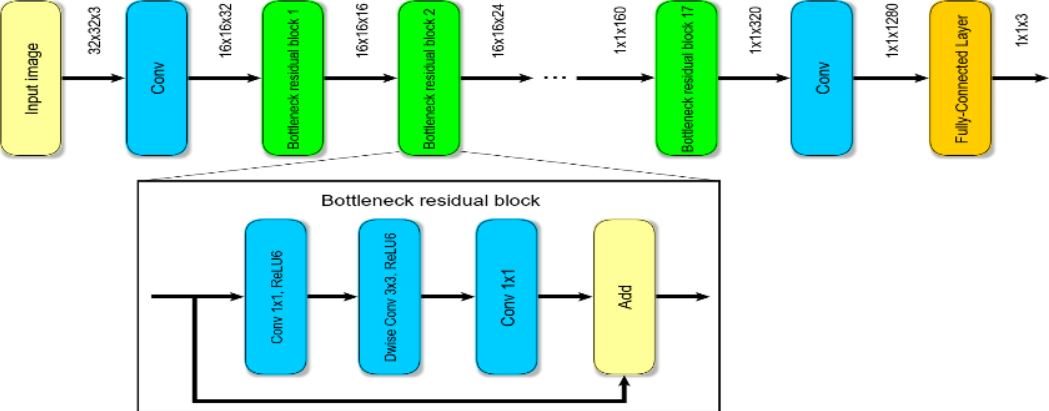
\includegraphics[width=1\textwidth]{obrazky-figures/mobilnetv2layers.png}
    \caption{The architecture of the MobileNetv2 network \cite{seidaliyeva2020layers}.}
    \label{fig:Mobilnetv2Architecture}
\end{figure}

A key component of MobileNetV2 is the inverted residual structure, which is a reversal of the traditional design where inputs and outputs are thin layers and expansion occurs in the middle. This design allows the network to maintain high accuracy while being computationally efficient. Depthwise separable convolutions are used to further reduce model size and computation cost without significantly affecting performance \cite{mobilnetv2}.

One of the defining characteristics of MobileNetV2 is its careful treatment of nonlinearities with the introduction of linear bottlenecks. By limiting the use of activation functions such as Rectified Linear Unit (ReLU) in the final layer of the bottleneck, important information is preserved, improving the efficiency of the network \cite{mobilnetv2}.

Additionally, MobileNetV2 employs transfer of knowledge to adapt pre-trained weights to gesture-specific tasks effectively. This approach reduces the need for extensive training data while still allowing the model to perform with high accuracy across different environments and scenarios. The efficient layer configuration of MobileNetV2 significantly helps in swiftly processing input gestures, thus supporting seamless and intuitive user experiences in real-time applications \cite{howard2019searching}.

\subsection{EfficientDet's Architecture}
EfficientDet is an innovative architecture designed primarily for efficient and scalable object detection, accommodating various computational constraints. This architecture embodies the integration of a compound scaling method and a novel bidirectional feature pyramid network (BiFPN), which significantly enhances multiscale feature fusion capabilities \cite{tan2020efficientdet}.

A key innovation in EfficientDet is the weighted BiFPN, which introduces learnable weights to assess the importance of different input features, enabling effective feature integration across multiple scales. This advancement addresses the challenge of efficiently combining multiresolution inputs, which is crucial to improving detection accuracy \cite{tan2020efficientdet}.

In addition, EfficientDet utilizes a compound scaling method that uniformly scales the resolution, depth, and width of the network, optimizing performance across a spectrum of resource limitations. This method allows EfficientDet to achieve superior detection accuracy with fewer parameters and reduced computational complexity compared to prior models such as YOLOv3 and RetinaNet \cite{tan2020efficientdet}.

EfficientDet has been rigorously tested on various benchmarks and demonstrates state-of-the-art performance, particularly in environments where computational resources are a~limiting factor. Its ability to scale dynamically with different computational budgets makes it a versatile choice for deployment in diverse settings, from mobile devices to high-end servers \cite{tan2020efficientdet}.

\section{Loss Functions}
Loss functions constitute a fundamental component of machine learning algorithms, guiding the optimization process toward models that can accurately predict or classify data. These functions evaluate the discrepancy between the algorithm's predictions and the actual target values, serving as a measure of performance for the model. In essence, a loss function quantifies how well the model performs, with lower values indicating better performance and a closer match to the desired output. In the domain of machine learning, loss functions can be broadly categorized based on the type of learning task - classification, detection, or segmentation. For classification tasks, such as gesture recognition using MobileNetV2, loss functions such as cross-entropy measure the difference between the predicted probability distribution across classes and the actual distribution. In regression tasks, functions such as mean squared error calculate the average squared difference between predicted values and actual values, providing a straightforward metric for the accuracy of the prediction. In addition, the choice of the loss function can significantly influence the behavior of the learning algorithm. It dictates the direction and steps the algorithm takes during the training process to minimize errors \cite{Wang2020ComprehensiveSF}.

\subsection{MobilenetV2 default loss function - Cross-entropy}
Cross-entropy is a widely used loss function in machine learning, particularly in classification tasks. It measures the difference between two probability distributions ---- predicted and actual ---- and is effective in training models such as neural networks. Cross-entropy, often paired with softmax activation in neural networks, quantifies the ``distance'' between the predicted probability distribution and the actual distribution of labels. This function is especially powerful in significantly adjusting the model weights for mispredicted labels, thus accelerating learning and improving the accuracy of the model \cite{mao2023crossentropy, lucena2022structured}. Furthermore, advances such as structured entropy and tamed cross-entropy adapt and modify traditional cross-entropy to tackle specific challenges such as label noise and hierarchical class structures, enhancing robustness and performance across various scenarios \cite{martinez2018tamed, li2020gradient}. As shown in Figure~\ref{fig:cross_entropy}, the cross-entropy loss function is used to measure the disparity between the actual class labels and the predicted probabilities, fostering effective learning by adjusting the model's predictions towards the actual labels \cite{Wang2020ComprehensiveSF}.

\begin{figure}[h]
    \centering
    \[
    L(y, p(y|x)) = -\log P(y|x)
    \]
    \caption{Cross-entropy loss function, where $y$ is the actual distribution and $p$ is the predicted probability distribution. Adapted from \cite{Wang2020ComprehensiveSF}.}
    \label{fig:cross_entropy}
\end{figure}

\section{Optimizers}

Optimizers are crucial in the field of machine learning, particularly in deep learning, where they significantly influence the efficiency and effectiveness of training models. An optimizer is essentially an algorithm designed to adjust the parameters of a neural network to minimize the loss function. This process is pivotal, as it directly impacts the model's ability to learn from the data and perform accurately on unseen data. In deep learning, several optimizers have emerged, each with unique characteristics and mechanisms. The choice of an optimizer is not trivial and depends on the specific needs of the application, the nature of the data, and the type of neural network that is being used. Some of the widely used optimizers include Stochastic Gradient Descent (SGD), Adam, RMSprop, and AdaGrad, among others. Choosing the right optimizer can significantly affect the speed of training and the final performance of deep learning models. Each optimizer has its strengths and weaknesses, making it essential to understand the underlying mechanisms and how they align with the specific requirements of the machine learning task at hand
\cite{Perin2020Influence}.


\subsubsection{Strengths and Weaknesses}
\begin{itemize}
    \item \textbf{SGD:} Utilizes a stochastic approximation of gradient descent, updating parameters incrementally for each training example, which can cause fluctuations in the loss function due to high variance \cite{Perin2020Influence}.
    \item \textbf{Mini-batch SGD:} Improves basic SGD by processing a fixed number of samples (a~mini-batch) in each update, balancing computational efficiency with variance reduction \cite{Perin2020Influence}.
    \item \textbf{Momentum:} Accelerates SGD by integrating a momentum term, which helps navigate through local optima by adding a fraction of the previous update vector to the current one, thus enhancing the convergence speed \cite{Perin2020Influence}.
    \item \textbf{Nesterov Accelerated Gradient (NAG):} Refines the concept of momentum by calculating the gradient at an approximate future position of the parameters, thus controlling the update velocity and improving optimization precision \cite{Perin2020Influence}.
    \item \textbf{Adagrad:} Adapts learning rates to parameters based on their frequency, with smaller updates for frequent features. It eliminates the need to manually adjust the learning rate, but can lead to a decrease in updates over time \cite{Perin2020Influence}.
    \item \textbf{Adadelta:} An extension of Adagrad that seeks to reduce its monotonically decreasing learning rate by limiting the window of accumulated gradients, thus maintaining a~more consistent learning rate over time \cite{Perin2020Influence}.
    \item \textbf{RMSprop:} RMSprop is an optimizer that adjusts the learning rate by dividing it by an exponentially decaying average of squared gradients. This approach helps to overcome the rapid decrease in the learning rate seen in Adagrad, making it suitable for handling non-stationary problems and online settings \cite{Perin2020Influence}.
    \item \textbf{Adam:} Adam, or Adaptive Moment Estimation, combines ideas from RMSprop and momentum. It calculates adaptive learning rates for each parameter by considering the first and second moments of the gradients, allowing for effective handling of sparse gradients. This versatility makes Adam highly favored for deep learning applications \cite{Perin2020Influence}.
\end{itemize}

\newpage

\subsection{Visualization of Optimizer Performance}
An illustrative figure \ref{fig:optimizer_landscape} shows the trajectory of different optimizers in the landscape of loss function. This visualization helps to understand how different optimizers navigate toward the minimum of a complex loss function landscape.
\begin{figure}[ht]
    \centering
    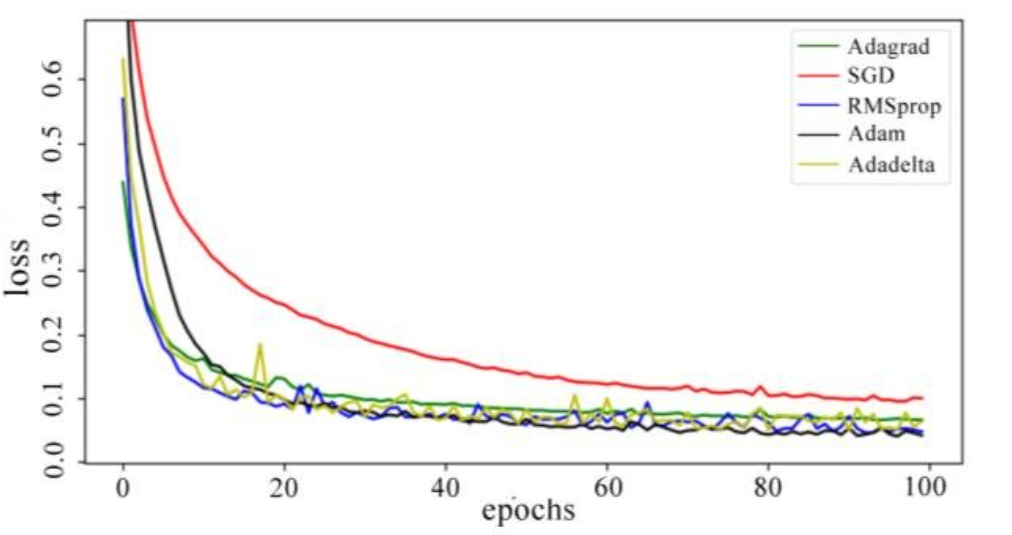
\includegraphics[width=0.8\textwidth]{obrazky-figures/optimizers_evaluation.png}
    \caption{Plot of the loss function over epochs during the training of the LSTM-CNN model for human activity recognition. The x-axis represents the number of epochs, while the y-axis represents the loss \cite{xia2020lstm}.}
    \label{fig:optimizer_landscape}
\end{figure}

These insights are crucial in selecting an optimizer that best fits the specific challenges and requirements of various deep learning tasks \cite{Perin2020Influence}.

\newpage

\subsection{SGD Optimizer}

Stochastic Gradient Descent (SGD) is a cornerstone of optimization in machine learning, especially in the training of deep neural networks. It updates the model parameters in the opposite direction of the gradient of the loss function concerning those parameters, with the goal of minimizing the loss. Although SGD in its pure form is simple, it serves as the foundation for more complex variants such as SGD with momentum and Nesterov-accelerated gradient (NAG), which aim to improve convergence rates and training stability. SGD and its derivatives are crucial for the optimization landscape in deep learning, offering a balance between computational efficiency and the ability to navigate the complex, high-dimensional loss surfaces typical of neural networks. Their simplicity, coupled with the nuanced understanding of their dynamics, makes them invaluable tools in the machine learning practitioner's toolkit
\cite{Perin2020Influence}.

\section{Quantization of a Model}
Model quantization is a crucial optimization technique to reduce the memory footprint and computational requirements of deep learning models, making them suitable for deployment on various platforms. The process involves converting the data formats of weights and activations from floating-point to lower-precision formats, such as 8-bit integers. This transformation can be performed in two primary ways: post-training quantization, which applies quantization after the model has been trained without the need for retraining; and quantization-aware training, which simulates low-precision arithmetic during the training process itself, thus retaining more of the model's accuracy \cite{Jacob2018}.

\chapter{Hardware and Software}
This chapter delves into the hardware and software aspect of running machine learning applications, namely the TensorFlow Lite, Keras, MobilnetV2 and the ARM architecture, with a particular focus on the i.MX 93 platform.

\section{ARM Architecture}
ARM architecture is pivotal in the realm of embedded systems, offering a robust framework for the efficient operation of myriad devices, from simple microcontrollers to complex SoCs (System on Chips). Originally developed as a project at Acorn Computers, ARM has grown to become the most widely used architecture in mobile devices, due to its power efficiency and performance optimization \cite{Dandamudi2005}.

\textbf{RISC Principles:} ARM is based on the RISC (Reduced Instruction Set Computing) design, which simplifies the instruction set, allowing for faster processing and lower power consumption compared to complex instruction set computing (CISC) designs. This simplicity is crucial for devices that require high performance with minimal energy expenditure \cite{Dandamudi2005}.

\textbf{Modularity and Customization:} ARM cores are highly modular, allowing hardware manufacturers to implement only the components necessary for their specific applications. This modularity extends to the inclusion of various coprocessors and a range of peripherals that can be tailored to specific needs, from automotive applications to mobile phones \cite{iMX93FAMFS}.

\textbf{Advancements in Technology:} Over the years, ARM has introduced several architectures and technologies that enhance the capability of systems in which they are embedded. Innovations such as ARM Cortex series, DynamIQ technology, and big.LITTLE processing not only provide scalable solutions but also integrate advanced processing capabilities like machine learning and artificial intelligence \cite{iMX93FAMFS}.

\textbf{Impact on Embedded Systems:} The application of ARM architecture extends beyond mobile phones to include automotive systems, industrial controls, and Internet of Things (IoT) devices. Its ability to support a range of operating systems from Linux to real-time operating systems underpins its versatility in handling various embedded system requirements \cite{iMX_LINUX_EMBEDDED}.

\section{i.MX 93}
The i.MX 93, which uses ARM architecture, represents a significant advancement in embedded systems, particularly for machine learning applications. It integrates the scalable Arm Cortex A55 core, which is critical for its best-in-class performance and energy efficiency. This core, enhanced by Arm's DynamIQ technology and the latest Armv8-A architecture extensions, is specifically optimized to accelerate machine learning tasks, making the i.MX 93 an ideal choice for Linux-based edge applications \cite{iMX93FAMFS}. Additionally, i.MX 93 is notable for its implementation of the Arm Ethos-U65 microNPU. As the first in the industry, the Ethos-U65 microNPU offers a blend of performance and efficiency, while maintaining an optimized footprint suitable for creating cost-effective and energy-efficient ML applications \cite{iMX93FAMFS}.

Apart from its advanced CPU and NPU capabilities, the i.MX 93 excels in power management and hardware versatility. Its innovative energy flex architecture enables fine-grained power control across heterogeneous domains, such as the application domain (Cortex-A55s), real-time domain (Cortex-M33 peripherals) and flex domains (NPU, DDR, etc.), ensuring minimal power consumption tailored to specific use cases \cite{iMX93FAMFS}. The platform also offers a comprehensive suite of high-speed interfaces and memory options, including USB, Ethernet, and CAN-FD, catering to a wide range of connectivity and data transfer needs \cite{iMX93FAMFS}. These features underscore the i.MX 93's potential in facilitating robust and efficient machine learning applications in embedded systems.

\section{TensorFlow Lite}
TensorFlow Lite is an open-source software library specifically designed to run machine learning models on mobile and embedded devices. \cite{tensorflow2015-whitepaper} It enables on-device machine learning inference with low latency and small binary size, making it ideal for embedded applications \cite{iMX_MACHINE_LEARNING_UG}. The version of TensorFlow Lite optimized for the NXP i.MX 8 and i.MX 93 platforms, as per the Yocto Linux release, includes features like multithreaded computation with acceleration using Arm Neon SIMD instructions on Cortex-A cores and parallel computation using NPU hardware acceleration \cite{iMX_MACHINE_LEARNING_UG}.

\section{Keras}
Keras is a high-level neural network API designed for rapid development and experimentation. It operates on top of several deep learning frameworks, including TensorFlow, which provides the backbone for building and training sophisticated machine learning models. Keras simplifies the process of building models through its user-friendly `Sequential` and functional API methods, supporting a wide range of network architectures from simple to complex. It is well suited for beginners and experienced researchers alike, offering easy model construction, evaluation, and deployment on a wide range of platforms, thus improving productivity and facilitating innovation \cite{chollet2015keras}.

\subsection{Epoch and Batch}
In the neural network training process, particularly in frameworks such as Keras, the terms epoch and batch are critical to understanding how models learn from data over iterations. An epoch represents one complete pass of the training dataset through the algorithm, allowing the model to learn from each example in the dataset. Each epoch consists of several smaller subsets of the data, known as batches, which are used to perform training iterations. A batch refers to the number of training examples used in one iteration of model training. The size of a batch and the number of epochs are adjustable parameters that can significantly affect the training dynamics and performance of the model. Batch processing in neural networks helps to efficiently manage computational resources, as using smaller batches means less memory consumption and often faster processing. However, smaller batches can lead to a less accurate estimate of the gradient, while larger batches provide a more stable gradient but with a higher computational cost. Adjusting the number of epochs is equally important, as it determines how many times the learning algorithm will work through the entire training dataset. Too few epochs can result in an underfit model, whereas too many epochs may lead to overfitting. It is crucial to find a balance to achieve optimal performance \cite{aldin2022accuracy}.


\section{AI on Embedded Systems}
\label{sec:ai_embedded_systems}
Implementing artificial intelligence in ARM-based embedded systems involves optimizing AI models for low power, limited hardware environments. TensorFlow Lite and MobileNetV2 are pivotal in this context due to their tailored design for such constraints. MobileNetV2, known for its lightweight deep neural network architecture, utilizes depthwise separable convolutions which significantly reduce the number of parameters and computational complexity, making it ideal for real-time applications on embedded devices \cite{mobilnetv2}.

\subsection{Optimizations for Efficient AI on ARM with TensorFlow Lite}
TensorFlow Lite facilitates optimizations through techniques such as post-training quantization and the use of fused operations, which streamline the computational graph. Furthermore, TensorFlow Lite's integration with the NXP board's specific hardware accelerators allows for enhanced processing capabilities, leveraging features such as the NEON SIMD architecture for parallel data processing \cite{tensorflow2015-whitepaper}.

These strategies collectively enable efficient deployment of MobileNetV2 on ARM-powered NXP boards, maintaining a balance between performance and power consumption, crucial for mobile and embedded applications.

\chapter{Analysis of Current Gesture Recognition Methods}
\section{Overview of Existing Gesture Recognition Techniques}

Gesture recognition technology has evolved significantly, employing various methods to interpret human gestures as a means of interaction with devices. This section explores various existing techniques, each with unique mechanisms and applications.

\subsection{Optical Gesture Recognition}
This method relies on cameras and computer vision algorithms that process visual data from a 2D or 3D perspective to detect and interpret gestures. Optical systems utilize depth-sensing technologies and computer algorithms to analyze the shape, movement, and depth of gestures within a given space, making it possible to interpret complex hand and body movements without physical contact. Such capabilities are critical in environments where intuitive user interfaces are necessary, such as in interactive or gaming systems \cite{segen1998fast}.

Despite seeming like a relatively modern development, optical gesture recognition has roots going back to at least 1997. Earlier systems, such as the one developed by Kobayashi, used CCD cameras and holographic devices to create vector representations of gestures. These early efforts laid the foundation for modern and more sophisticated systems, demonstrating the long-standing interest and continuous evolution in the field of gesture recognition \cite{kobayashi1997optical}.

\subsection{Sensor Gloves}
Sensor-equipped gloves are another approach, where the glove is embedded with various sensors such as accelerometers, gyroscopes, and sometimes flex sensors. These gloves can capture the fine movements and positions of the user's fingers and hand, translating them into control signals. Although offering high accuracy, the requirement to wear a glove can be seen as a limitation in terms of convenience and scalability. Such systems have been effectively demonstrated to help in gesture recognition for communication, especially in applications where precise control is necessary, such as interacting with virtual environments \cite{preetham2013hand}.

\subsection{Touch-Based Gesture Recognition}
Predominantly found in smartphones and tablets, this method uses capacitive touchscreens to recognize gestures. Simple gestures such as swipes, pinches, and taps are easily recognized. Despite their widespread adoption, the interaction is limited to the two-dimensional plane of the screen while requiring direct contact with the device, which limits the type of gestures that can be recognized and may not capture more complex three-dimensional gestures intended for advanced computational interactions \cite{panella2019smartphone}.

\subsection{Wearable Device-Based Recognition}
Wearable devices such as smartwatches and fitness bands use embedded sensors to recognize gestures. These devices primarily use accelerometers and gyroscopes to understand simple hand movements. Although convenient and increasingly popular, the range of recognizable gestures is relatively limited compared to more sophisticated systems. The embedded sensors in these devices allow for recognition of a variety of gestures by analyzing movements of the wrist, which can be crucial for applications that require user-friendly and intuitive interfaces \cite{xu2015finger}.

\subsection{Infrared and Ultrasonic Gesture Recognition} These techniques use infrared sensors or ultrasonic wave emissions to detect hand movements. By measuring the time it takes for waves to bounce back from the hand, the system interprets different gestures. Such methods can be effective for short-range interactions, but might struggle with precision and complex gesture interpretation \cite{rahulnath2019gesture}.

\section{Advantages of Gesture Recognition Compared to Traditional Control Methods}

Gesture recognition technology offers several advantages over traditional control methods such as physical buttons, touchscreens, and control sticks. This section highlights the key benefits of using gesture-based interfaces.

\subsection{Intuitive and Natural Interaction}
One of the primary advantages of gesture recognition is its ability to provide a more intuitive and natural way of interaction. Unlike pressing buttons or using a~mouse, gestures are a~fundamental form of human communication, often perceived as more natural and intuitive. Studies have shown that users can perform tasks more quickly and with fewer errors using gestures compared to traditional interfaces \cite{Choi2014}.

\subsection{Enhanced Accessibility}
Gesture-based interfaces can be more inclusive, especially for people with disabilities. For those who may find it challenging to use traditional interfaces due to physical limitations, gesture recognition can offer an alternative means of interaction, as demonstrated in research on accessible technology \cite{Choi2014}.

\subsection{Contactless Control}
In scenarios where touchless control is preferable or required for hygiene reasons (like in medical settings or public kiosks), gesture recognition provides an effective solution. This contactless nature also makes it suitable for use in environments where touchscreens or buttons can be prone to damage \cite{Ye2018}.

\subsection{Freedom of Movement}
Gesture recognition allows for greater freedom of movement, eliminating the need to be physically close to the device. This can be particularly beneficial in situations such as presentations or interactive installations, where the user can control the system from a~distance \cite{ZhiHeng2017}.

\subsection{Space and Cost Efficiency}
Implementing gesture control can lead to more space-efficient designs, as it reduces the need for physical control panels and buttons. This can also translate into cost savings in design and manufacturing \cite{Choi2014}.

\subsection{Scalability and Versatility}
Gesture recognition technology can be scaled and adapted to a wide range of applications, from consumer electronics to industrial control systems. Its versatility allows it to be implemented in diverse environments and for various purposes \cite{Jha2018}.

\subsection{Reduced Wear and Tear}
Since gesture-based interfaces do not require physical contact, they typically experience less wear and tear compared to traditional control methods. This can lead to longer-lasting devices and a less frequent need for maintenance or replacement \cite{Yan2012}.

\section{Current Challenges and Limitations in Gesture Recognition}

Despite its many advantages, gesture recognition technology also faces several challenges and limitations that affect its broader adoption and effectiveness.

\subsection{Environmental Sensitivity}
Gesture recognition systems, especially those based on optical or infrared technologies, can be highly sensitive to environmental factors. Lighting conditions, background clutter, and interference or even color of the skin of a human being from other sources can significantly impact the accuracy of gesture detection \cite{Choi2014}.

\subsection{Complexity of Gesture Interpretation}
Interpreting complex gestures accurately remains a challenge. Different individuals may perform the same gesture slightly differently, and the system must be able to account for these variations. Furthermore, technology must distinguish between intentional gestures and random movements \cite{Escalera2016}.

\subsection{Hardware Limitations}
The effectiveness of gesture recognition is often limited by hardware capabilities. High resolution sensors and advanced processing capabilities are required for precise gesture detection, which can be costly and power consuming, especially for portable or wearable devices \cite{Iyer2016}.

\subsection{User Acceptance and Adaptability}
User acceptance can be a significant barrier, as some may find it uncomfortable or unintuitive to use gesture-based controls, especially in public or professional settings. There is also a learning curve associated with adopting new interaction methods \cite{Si2022}.

\subsection{Privacy and Security Concerns}
Camera-based gesture recognition systems raise privacy concerns, as continuous monitoring and video recording might be perceived as intrusive. Furthermore, ensuring the security of gesture data is critical to prevent unauthorized access or control \cite{Wu2023}.

\subsection{Lack of Standardization}
There is a lack of standardization in gestures and gesture recognition technologies, leading to inconsistencies between different systems and devices. This can confuse users and hinder the interoperability between different systems and applications \cite{Li2022}.

\chapter{Training a Machine Learning Model for Optical Gesture Recognition}

\section{Used Models}

In this project, two distinct models were utilized to address the challenge of gesture recognition. MobileNetV2 and EfficientDet Lite 2. Both models are well-regarded for their performance in computer vision tasks and have been adapted to meet the specific requirements of real-time gesture recognition on embedded systems.

\section{Dataset Description}
The dataset, sourced from a GitHub repository HaGRID \cite{hagrid}, comprises a diverse collection of images used to train the machine learning model consisting of 19 different hand gestures \ref{fig:dataset_gestures}. It contains around 554,800 unique persons \ref{fig:dataset_examples} and at least an equal number of unique scenes. The subjects range in age from 18 to 65 years, offering a broad demographic representation. The data set was collected primarily indoors with considerable variation in lighting conditions, encompassing artificial and natural light sources. It also includes images taken under challenging lighting conditions, such as with subjects facing or backing to a window. Furthermore, the dataset captures gestures performed at varying distances, from 0.5 to 4 meters from the camera, adding to the complexity and diversity of the data used for training the model. This variety ensures that the model is trained in a wide range of scenarios, enhancing its robustness and applicability in real world settings.
\newpage
\begin{figure}[h]
    \centering
    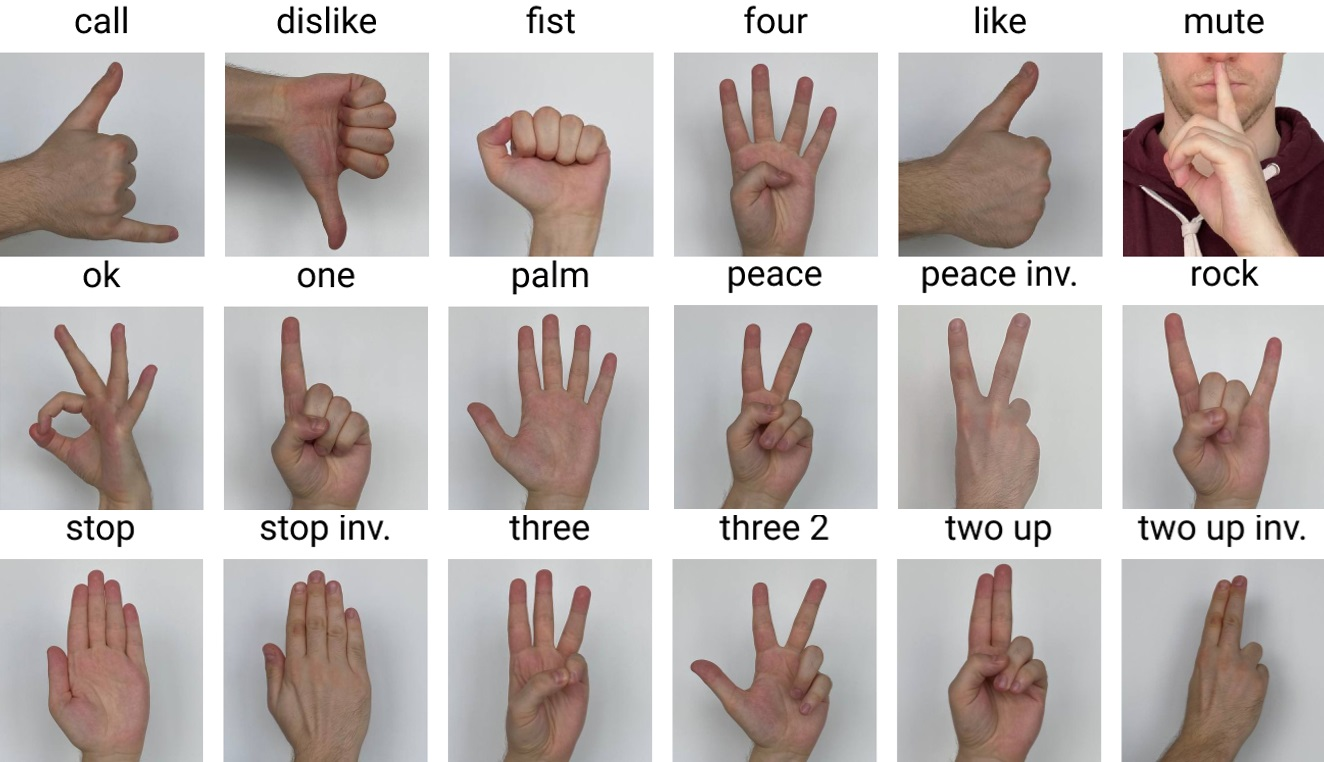
\includegraphics[width=0.6\textwidth]{obrazky-figures/gestures_jpg.jpg}
    \caption{Gestures from the HaGRID dataset}
    \label{fig:dataset_gestures}
\end{figure}

\begin{figure}[h]
    \centering
    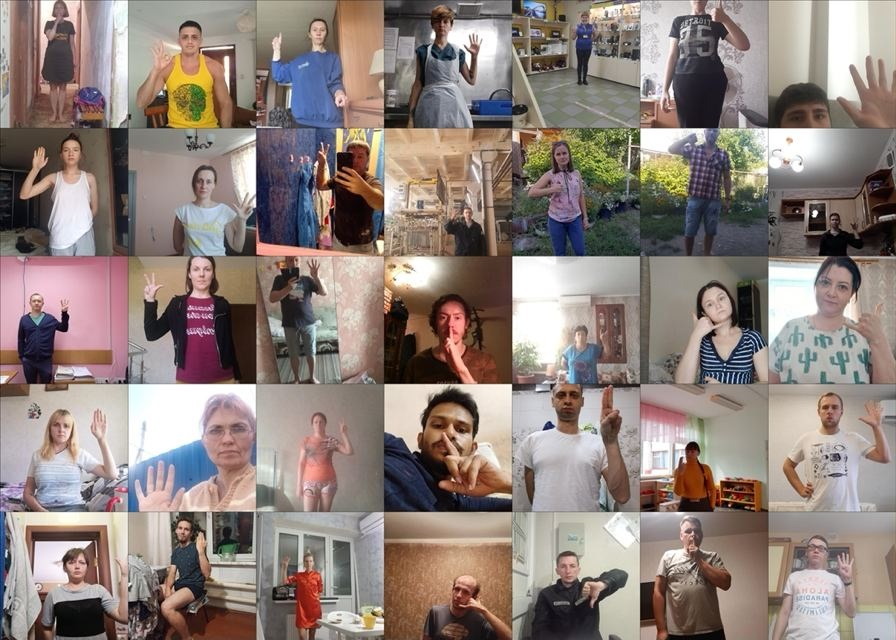
\includegraphics[width=0.9\textwidth]{obrazky-figures/data_set_example.jpg}
    \caption{Examples of images from the HaGRID dataset}
    \label{fig:dataset_examples}
\end{figure}

\newpage
\subsection{Dataset Preprocessing}
The initial dataset sourced from a GitHub repository contained a wide variety of hand gestures. To enhance the accuracy and focus of the machine learning model and simplify real life usage of device control via gesture recognition, the dataset was curated to include only five gestures that are distinctly different from each other. These gestures-like, dislike, fist, peace, and stop --were selected to provide clear and varied examples for the model to learn from, thereby improving its ability to accurately classify these gestures.

From the repository, I extracted 140 images for each of these five gestures. Then each image was manually cropped to focus solely on the gesture, ensuring that each cropped image maintained a resolution of 224x224 pixels. This specific resolution was chosen to comply with the input requirements of the MobileNetV2 model, which is optimized for this image size due to its architectural constraints and operational efficiency.

The dataset was strategically divided to enhance the training and validation processes: 100 images per gesture were designated for training, while 20 images per gesture were set aside for validation, and another 20 for testing. This division was aimed at providing a~balanced approach to training the model while allowing for comprehensive validation and testing to assess the model performance accurately.

For the EfficientDet Lite 2 model, an additional set of 140 images was utilized for each gesture. However, for this model, the original annotations from the dataset were retained and converted from the COCO format to the VOC format, which is compatible with the model's training requirements. This approach allowed for leveraging the pre-annotated data effectively, reducing the preprocessing workload while maintaining high data integrity for training the second model. This method ensured that both models were trained under optimal conditions with datasets tailored to their specific needs, with the aim of maximizing the accuracy and effectiveness of the gesture recognition system.


\subsection{Dataset Augmentation}
Data augmentation involves artificially altering the training dataset by applying random, yet realistic, transformations to the training images. For the MobileNetV2 model, a variety of augmentations were used to ensure that the model is not only accurate, but also robust to variations in real-world conditions. These alterations are being performed every epoch on every image randomly.

\paragraph{MobileNetV2 Augmentations}
The training dataset for MobileNetV2 was augmented using the following transformations:
\begin{itemize}
    \item \textbf{Rescaling}: Each pixel value was rescaled by a factor of \(\frac{1}{255}\), converting the pixel values from a range of 0-255 to 0-1. This normalization helps speed up the training by improving numerical stability.
    \item \textbf{Shear Transformation}: A shear range of 0.2 was applied, which slants the shape of the image, simulating a more diverse set of angles and poses in captured gestures.
    \item \textbf{Zoom}: The images were randomly zoomed in by up to 20\%, helping the model to recognize gestures from various scales and distances.
    \item \textbf{Horizontal Flip}: Horizontal Flip was utilized because it allows the model to learn from mirrored versions of gestures. This is particularly beneficial because a gesture shown on the left hand can be transformed to simulate how it would appear if performed with the right hand, thereby doubling the diversity of hand orientation in the training data without needing additional images.
    \item \textbf{Rotation}: The images were randomly rotated by up to 30 degrees, allowing the model to handle variations in the wild where gestures might not be perfectly aligned with the camera.
\end{itemize}

\paragraph{Limitations with EfficientDet Lite 2}
In contrast, the augmentation capabilities of EfficientDet Lite 2 were limited by the tools available within the TensorFlow Lite Model Maker environment used for training. Although MobileNetV2 training could leverage direct image augmentation through Keras, which provides extensive support for image augmentation through its \texttt{ImageDataGenerator} class, EfficientDet Lite 2 did not support similar on-the-fly augmentations directly in its training pipeline at the time of implementation. The setup for EfficientDet Lite 2 required predefined datasets with less flexibility in augmentation, illustrating a trade-off between ease of use and flexibility in training deep learning models for gesture recognition.

\section{Implementation Details}
\subsection{Code Overview}
The implementation comprises Python and Bash scripts for various stages such as training, data augmentation, annotation filtering, and converting the model to TensorFlow Lite format \cite{gajdosik2024gesture}. The TensorFlow and Keras libraries were employed for training, utilizing the pre-trained layers of MobileNetV2 and adding custom layers tailored for the specific task. MobileNetV2 was initially trained; however, attempts to quantize this model were unsuccessful. Due to difficulties encountered during the quantization process, MobileNetV2 could not be effectively prepared for deployment on Neural Processing Units (NPU). Consequently, the EfficientDet Lite 2 model was trained and subsequently quantized successfully, ensuring compatibility and efficient execution on NPU platforms.

\subsection{Software Dependencies}
The project's software dependencies are tailored to ensure compatibility and performance for machine learning development, particularly on x64 platforms using Ubuntu 22.04. The dependencies are as follows:

\begin{itemize}
\item \textbf{Python Version: 3.10.12} - Chosen for its stability and compatibility with other libraries required in this project.
\item \textbf{TensorFlow 2.15} - TensorFlow 2.15 supports legacy functionalities with Keras 2, which were used in the initial stages of this project. While TensorFlow 2.16 was released during the development process, it was not adopted to ensure stability and compatibility with the existing codebase, which is tailored for TensorFlow 2.15.
\item \textbf{Keras 2} - Integrated directly within TensorFlow 2.15 to leverage specific legacy features not available in later versions.
\item \textbf{OpenCV-Python (cv2)} - Utilized for handling image and video data, essential for data preprocessing and augmentation tasks.
\end{itemize}

The combination of Python, TensorFlow, and OpenCV-Python creates a powerful and versatile development environment. This setup is ideal for meeting the project's demands in terms of processing speed and data handling. The environment ensures compatibility and high performance across x64 platforms, providing a robust foundation for the development and testing phases of the machine learning models.

\section{Training Process of MobileNetV2}

\subsection{Loading the MobileNetV2 model without top layers}
At the beginning of the training process, the pre-trained MobileNetV2 model was loaded without its top classification layers \ref{code:mobilenet_loading}. This approach allows for leveraging the learned features while adapting the model to a new classification task with fewer output categories.

\begin{figure}[H]
\begin{lstlisting}[language=Python]
import tensorflow as tf
model = tf.keras.applications.MobileNetV2(weights='imagenet', include_top=False, input_shape=(224, 224, 3))
\end{lstlisting}
\caption{Loading the MobileNetV2 model without top layers}
\label{code:mobilenet_loading}
\end{figure}

\subsection{Freezing the layers of the MobileNetV2 model}
The rest of the layers of the pre-trained MobileNetV2 model were frozen to prevent them from being updated throughout the training process \ref{code:freeze_layers}. This strategy is used to preserve the intricate features that the model has learned from the comprehensive ImageNet dataset. By keeping these layers fixed, only the newly added custom layers are trained, allowing the model to specialize on the narrower task without forgetting the valuable generalized features.

\begin{figure}[H]
\begin{lstlisting}[language=Python]
for layer in model.layers:
    layer.trainable = False
\end{lstlisting}
\caption{Freezing the layers of the MobileNetV2 model}
\label{code:freeze_layers}
\end{figure}

\subsection{Adding custom layers to the MobileNetV2 model}
After loading and configuring the base model, custom layers were added to tailor the model for our specific classification tasks \ref{code:custom_layers}. These layers include a global average pooling layer which computes the average output of each feature map from the previous layer followed by a dense layer for feature reduction and a final dense layer with softmax activation for classification.

\begin{figure}[H]
\begin{lstlisting}[language=Python]
from tensorflow.keras import layers, models
x = model.output
x = layers.GlobalAveragePooling2D()(x)
x = layers.Dense(1024, activation='relu')(x)
predictions = layers.Dense(5, activation='softmax')(x)
model_final = models.Model(inputs=model.input, outputs=predictions)
\end{lstlisting}
\caption{Adding custom layers to the MobileNetV2 model}
\label{code:custom_layers}
\end{figure}

\subsection{Compiling the MobileNetV2 model with SGD optimizer}
The model was then compiled with a stochastic gradient descent (SGD) optimizer, specifying the learning rate and the momentum \ref{code:compile_model}. This sets up the model for training by defining how it should update its weights (via the optimizer) and how it should measure its accuracy (via the loss function and other metrics). The learning rate and momentum values were chosen as the best after numerous iterative experiments with different values.

\begin{figure}[H]
\begin{lstlisting}[language=Python]
from tensorflow.keras.optimizers import SGD
optimizer = SGD(learning_rate=0.001, momentum=0.9)
model_final.compile(optimizer=optimizer, loss='categorical_crossentropy', metrics=['accuracy'])
\end{lstlisting}
\caption{Compiling the MobileNetV2 model with SGD optimizer}
\label{code:compile_model}
\end{figure}

\subsection{Setting up data augmentation with ImageDataGenerator}
During the training phase, a data augmentation strategy was implemented to enhance the model's ability to generalize to new unseen data \ref{code:data_augmentation}. This strategy was executed using an instance of the \texttt{ImageDataGenerator} class provided by TensorFlow's Keras API, which applies various transformations to the training images.

\begin{figure}[H]
\begin{lstlisting}[language=Python]
train_datagen = ImageDataGenerator (
    rescale=1./255,
    shear_range=0.2,
    zoom_range=0.2,
    horizontal_flip=True,
    rotation_range=30,
)
\end{lstlisting}
\caption{Setting up data augmentation with ImageDataGenerator}
\label{code:data_augmentation}
\end{figure}

\subsection{Specifying batch size and training dimensions}
Training was carried out with a batch size of 32 \ref{code:training_params}, since this value produced the best training speed for both MobileNetV2 and EfficientDet Lite 2. The value of 20 for the number of epochs to be trained was chosen because the autostopper with default values for the MobilnetV2 model always stopped at 20 epochs after not being able to improve the model with more epochs. To preserve the same value baseline for both models, this number was also chosen for EfficientDet Lite 2.

\begin{figure}[H]
\begin{lstlisting}[language=Python]
batch_size = 32
epochs = 20
img_height, img_width = 224, 224
\end{lstlisting}
\caption{Specifying batch size and training dimensions}
\label{code:training_params}
\end{figure}

\subsection{Converting the trained model to TensorFlow Lite format}
Following model training, the TensorFlow model was converted to TensorFlow Lite format \ref{code:model_conversion}, enabling its deployment on the i.MX 93 board.

\begin{figure}[H]
\begin{lstlisting}[language=Python]
import tensorflow as tf
converter = tf.lite.TFLiteConverter.from_keras_model(model)

tflite_model = converter.convert()
with open('model.tflite', 'wb') as f:
    f.write(tflite_model)
\end{lstlisting}
\caption{Converting the trained model to TensorFlow Lite format}
\label{code:model_conversion}
\end{figure}

\newpage
\section{Training Process of EfficientDet Lite 2}

The training process for the EfficientDet Lite 2 model began by initializing the model with pre-set specifications \ref{code:init_efficientdet_lite2} tailored for lightweight and efficient performance on mobile devices.

\begin{figure}[H]
\begin{lstlisting}[language=Python]
import tensorflow as tf
from tflite_model_maker import model_spec
spec = model_spec.get('efficientdet_lite2')
\end{lstlisting}
\caption{Initializing the EfficientDet Lite 2 model}
\label{code:init_efficientdet_lite2}
\end{figure}

\subsection{Loading training and validation data for EfficientDet Lite 2}
Data for training and validation were loaded using TensorFlow Model Maker's DataLoader \ref{code:data_loading_efficientdet_lite2}, which organizes images and annotations from the Pascal VOC format, commonly used for object detection tasks.

\begin{figure}[H]
\begin{lstlisting}[language=Python]
from tflite_model_maker import object_detector
train_data = object_detector.DataLoader.from_pascal_voc(
    images_dir="dataset_train", annotations_dir="annotations_train", label_map={1:"dislike", 2:"fist", 3:"like", 4:"peace", 5:"stop"}, num_shards=10
)
validation_data = object_detector.DataLoader.from_pascal_voc(
    images_dir="dataset_val", annotations_dir="annotations_val", label_map={1:"dislike", 2:"fist", 3:"like", 4:"peace", 5:"stop"}, num_shards=10
)
\end{lstlisting}
\caption{Loading training and validation data for EfficientDet Lite 2}
\label{code:data_loading_efficientdet_lite2}
\end{figure}

\subsection{Configuring and starting training for EfficientDet Lite 2}
Training was carried out with a batch size of 32 with 20 epochs \ref{code:train_efficientdet_lite2}, as these values yielded the best ratio of training speed and mode accuracy for both models. The value of 20 for the number of epochs to be trained was also chosen because the autostopper with default values for the MobilnetV2 model always stopped at 20 epochs after not being able to improve the model with more epochs. To preserve the same value baseline for both models, this number was also chosen for EfficientDet Lite 2.

\begin{figure}[H]
\begin{lstlisting}[language=Python]
model = object_detector.create(train_data,
    model_spec=spec, batch_size=32, epochs=20, train_whole_model=True, validation_data=validation_data)
\end{lstlisting}
\caption{Configuring and starting training for EfficientDet Lite 2}
\label{code:train_efficientdet_lite2}
\end{figure}

\subsection{Quantizing the EfficientDet Lite 2 model}
After training, the model was quantized \ref{code:quantization_efficientdet_lite2}, which optimizes it for deployment by reducing the size of the model and potentially improving its speed on compatible hardware. The quantization settings were specified to use INT8 precision for inference.

\begin{figure}[H]
\begin{lstlisting}[language=Python]
from tflite_model_maker.config import QuantizationConfig
config = QuantizationConfig.for_int8(validation_data, inference_input_type=tf.uint8, inference_output_type=tf.float32, supported_ops=[tf.lite.OpsSet.TFLITE_BUILTINS_INT8])
\end{lstlisting}
\caption{Quantizing the EfficientDet Lite 2 model}
\label{code:quantization_efficientdet_lite2}
\end{figure}

\subsection{Exporting the EfficientDet Lite 2 model in TensorFlow Lite format}
Finally, the model was exported in TensorFlow Lite format \ref{code:export_tflite_efficientdet_lite2}, allowing its deployment on the i.MX 93 board.

\begin{figure}[H]
\begin{lstlisting}[language=Python]
model.export(export_dir='.', tflite_filename="model.tflite", quantization_config=config)
\end{lstlisting}
\caption{Exporting the EfficientDet Lite 2 model in TensorFlow Lite format}
\label{code:export_tflite_efficientdet_lite2}
\end{figure}

\subsection{Optimizing the Quantized EfficientDet Lite 2 Model for NPU}
Once the EfficientDet Lite 2 model was quantized and saved in TensorFlow Lite format, using Vela Tool, the quantized `.tflite` model undergoes further transformation that refines the model for optimal execution on the NPU. This includes restructuring certain layers and operations to better exploit the parallel processing capabilities of NPUs.

The command to run Vela on the quantized model is straightforward \ref{code:vela_optimization}. Suppose that Vela Tool is installed and configured on the system.

\begin{figure}[H]
\begin{lstlisting}[language=bash]
vela model.tflite
\end{lstlisting}
\caption{Using Vela Tool to optimize the TensorFlow Lite model for NPU execution}
\label{code:vela_optimization}
\end{figure}

\chapter{Inference Process}

\section{Code Overview}
The inference process involves loading the TensorFlow Lite model and processing input data \cite{gajdosik2024gesture}, typically from a USB camera connected to the i.MX 93's board or from a video file. On the x64 platform, the inference can be run on CPU or on supported GPUs from NVIDIA. On ARM platform, the i.MX 93's CPU cores or NPU or both at the same time can handle the inference, demonstrating the board's capability to perform real-time machine learning tasks. The inference script includes preprocessing of the input data, model invocation, and output of the predictions.

\subsection{Software Dependencies}
The script requires specific libraries and environments to run efficiently. The dependencies are outlined as follows:

\subsubsection{Inference on x64 platform}

\begin{itemize}
    \item \textbf{Python Version: 3.10.12} - Chosen for its stability and compatibility with other libraries required in this project.
    \item \textbf{TensorFlow 2.15} - TensorFlow 2.15 is the version the models were trained in and as to have continuity, this version is also required for inference even though the inference script has no issues with the newest TensorFlow version 2.16.
    \item \textbf{OpenCV-Python (cv2)} - Utilized for handling image and video data.
    \item \textbf{NumPy} - Utilized for numerical operations on image data.
\end{itemize}

\subsubsection{Inference on ARM platform}
The inference process on ARM platforms, particularly using i.MX 93, is streamlined by the dedicated version of Embedded Linux customized for this device. The specific version \textbf{Embedded Linux for i.MX applications processors 6.1.36\_2.1.0 \cite{iMX_LINUX_EMBEDDED}}, released on \textbf{December 1, 2023}, includes all the necessary dependencies and libraries required to efficiently run inference tasks directly out of the box and is tested and compatible with the project's inference code and trained models.

This Linux release is readily available for download from the NXP website following a simple registration process. Not only does it offer the operating system, but also it provides comprehensive documentation that assists developers in deploying and optimizing their applications. The integration of all required software components within this Linux version ensures that developers can quickly set up their inference environment without needing to manually install additional packages. This feature is especially beneficial in embedded systems, where simplicity and efficiency are crucial. For more detailed guidance on setting up and using this Linux release, refer to the accompanying user guide \cite{iMX_LINUX_USERS_GUIDE}.

\section{Detailed Implementation}

\subsection{Parsing Arguments}
The script starts by defining and parsing command-line arguments \ref{code:arg_parsing}, which allow the user to customize the execution parameters directly from the command line. This flexibility is essential for adapting the script to different environments and input types. After parsing, the script loads these arguments into local variables, which are then used to configure the execution environment and the path setup for the model file.

\begin{figure}[H]
\begin{lstlisting}[language=Python]
# Define and parse input arguments
parser = argparse.ArgumentParser()
parser.add_argument('--filename', help='Name of video or image input file',
                    default='video_device.mp4')
parser.add_argument('--graph', help='Name of the .tflite file, if different than model.tflite',
                    default='model.tflite')
parser.add_argument('--input_type', help='Type of input: webcam, videofile',
                    default='webcam')
parser.add_argument('--platform', help='Type of platform: arm, x64',
                    default='arm')
args = parser.parse_args()

# Load args
inputFile = args.filename
GRAPH_NAME = args.graph
inputType = args.input_type
platformType = args.platform

# Get path to current working directory
CWD_PATH = os.getcwd()
# Path to .tflite file, which contains the model that is used for object detection
model_path = os.path.join(CWD_PATH,GRAPH_NAME)
\end{lstlisting}
\caption{Parsing command-line arguments and loading them into the script}
\label{code:arg_parsing}
\end{figure}

In example, if we wanted to infer on the x64 platform, with model named ''mobilnetv2.tflit'' on input from mp4 video named video\_test.mp4 we would run the script with command described in the following figure \ref{code:arg_example}.

\begin{figure}[H]
\begin{lstlisting}[language=Bash]
python3 inference_mobilnetv2.py 
    --platform      x64
    --input_type    videofile
    --filename      video_test.mp4
    --graph         mobilnetv2.tflite
\end{lstlisting}
\caption{Arguments example}
\label{code:arg_example}
\end{figure}

\subsection{Importing Libraries}
Depending on the platform (x64 \ref{code:import_libraries} or ARM \ref{code:import_libraries_arm}), the appropriate TensorFlow Lite library is imported to ensure compatibility. If we want to make an inference on the NPU of i.MX 93, we need to decide whether we also want to import a loader for a delegate \ref{code:import_libraries_arm_npu}.

\begin{figure}[H]
\begin{lstlisting}[language=Python]
import tensorflow as tf
interpreter = tf.lite.Interpreter(model_path=model_path)
\end{lstlisting}
\caption{Importing x64 library}
\label{code:import_libraries}
\end{figure}

\begin{figure}[H]
\begin{lstlisting}[language=Python]
from tflite_runtime.interpreter import Interpreter
interpreter = Interpreter(model_path=model_path)

\end{lstlisting}
\caption{Importing arm library}
\label{code:import_libraries_arm}
\end{figure}

\begin{figure}[H]
\begin{lstlisting}[language=Python]
from tflite_runtime.interpreter import Interpreter
from tflite_runtime.interpreter import load_delegate
ext_delegate = [load_delegate("/usr/lib/libethosu_delegate.so")]
interpreter = Interpreter(model_path=model_path, experimental_delegates=ext_delegate)
\end{lstlisting}
\caption{Importing delegate library}
\label{code:import_libraries_arm_npu}
\end{figure}

\subsection{Initializing the TensorFlow Lite Interpreter}
At the outset, the TensorFlow Lite interpreter is initialized to facilitate the execution of the pretrained machine learning model. This step is crucial because it prepares the interpreter to process the input data through the model by loading the model architecture and weights from the compiled TensorFlow Lite file \ref{code:init_interpreter}.

\begin{figure}[H]
\begin{lstlisting}[language=Python]
interpreter.allocate_tensors()
input_details = interpreter.get_input_details()
output_details = interpreter.get_output_details()
\end{lstlisting}
\caption{Initializing the TensorFlow Lite interpreter}
\label{code:init_interpreter}
\end{figure}

\subsection{Setting up Video Capture Based on the Input Type}
This step configures the video capture based on the input type specified: a webcam or a pre-recorded video file \ref{code:video_input}. The script checks if the video capture device can be opened successfully, ensuring that the input source is ready for frame extraction and processing.

\begin{figure}[H]
\begin{lstlisting}[language=Python]
if input_type == 'webcam':
    cap = cv2.VideoCapture(0)
else:
    cap = cv2.VideoCapture(input_file)

if not cap.isOpened():
    print("Error: Could not open video or webcam.")
    exit(1)
\end{lstlisting}
\caption{Setting up video capture based on the input type}
\label{code:video_input}
\end{figure}

\subsection{Preprocessing Frames}
During this stage, each frame captured from the video source undergoes a series of transformations to meet the specific input requirements of different models. The frame is first cropped to the center to ensure that the focus remains on the main subject of the image. It is then resized according to the required input dimensions of the model: $448 \times 448$ pixels for the Efficientdet Lite 2 model and $224 \times 224$ pixels for the MobileNetV2 model.

For the Efficientdet Lite 2 model, frames are resized to larger dimensions and kept in an 8-bit unsigned integer format (uint8) which aligns with the model's architectural requirements for handling color depth and intensity directly, as shown in the first code snippet \ref{code:EfficientDet Lite 2_preprocess}.

For the MobileNetV2 model, the resized frames are additionally normalized to have pixel values between 0 and 1, converting the data type to a 32-bit floating point (float32). This normalization is crucial, as it scales down the pixel values, facilitating the model's learning and prediction processes by maintaining numerical stability and speeding up computation, as demonstrated in the second code snippet \ref{code:mobilenetv2_preprocess}.

\begin{figure}[H]
\begin{lstlisting}[language=Python]
def preprocess_frame(frame):
    min_dim = min(frame.shape[:2])
    start_x = (frame.shape[1] - min_dim) // 2
    start_y = (frame.shape[0] - min_dim) // 2
    cropped_frame = frame[start_y:start_y+min_dim, start_x:start_x+min_dim]
    resized_frame = cv2.resize(cropped_frame, (448, 448))
    return np.expand_dims(resized_frame, axis=0).astype(np.uint8), resized_frame
\end{lstlisting}
\caption{Preprocessing frames for EfficientDet Lite 2 model}
\label{code:EfficientDet Lite 2_preprocess}
\end{figure}

\begin{figure}[H]
\begin{lstlisting}[language=Python]
def preprocess_frame(frame):
    min_dim = min(frame.shape[:2])
    start_x = (frame.shape[1] - min_dim) // 2
    start_y = (frame.shape[0] - min_dim) // 2
    cropped_frame = frame[start_y:start_y+min_dim, start_x:start_x+min_dim]
    resized_frame = cv2.resize(cropped_frame, (224, 224))
    normalized_frame = resized_frame / 255.0
    return np.expand_dims(normalized_frame, axis=0).astype(np.float32), resized_frame
\end{lstlisting}
\caption{Preprocessing frames for MobileNetV2 model}
\label{code:mobilenetv2_preprocess}
\end{figure}

These preprocessing steps ensure that the input to each model is consistent and optimized for the best inference performance, taking into account the architectural nuances of each model.

\subsection{Performing Inference}
Once the frame is pre-processed, it is fed into the TensorFlow Lite model to perform inference. The method of extracting the prediction results varies slightly depending on the model used.

\subsubsection{MobileNetV2 Inference}
For the MobileNetV2 model, the processed frame tensor is set as input to the model \ref{code:mobilenetv2_inference}. The model then runs inference and outputs the prediction probabilities for each class.

\begin{figure}[H]
\begin{lstlisting}[language=Python]
interpreter.set_tensor(input_details[0]['index'], processed_frame)
interpreter.invoke()
predictions = interpreter.get_tensor(output_details[0]['index'])
\end{lstlisting}
\caption{Inference processing for MobileNetV2}
\label{code:mobilenetv2_inference}
\end{figure}

\subsubsection{EfficientDet Lite 2 Inference}
For the EfficientDet Lite 2 model, the inference process is similar in setting the tensor and invoking the model \ref{code:mobilenetv2_inference}. However, this model provides detailed outputs, such as the class indices of the detected objects that were set during training and their respective confidence scores \ref{code:edl2_inference}.

\begin{figure}[H]
\begin{lstlisting}[language=Python]
interpreter.set_tensor(input_details[0]['index'], processed_frame)
interpreter.invoke()
classes = interpreter.get_tensor(output_details[3]['index'])[0]  % Class index
probabilities = interpreter.get_tensor(output_details[0]['index'])[0]  % Confidence
\end{lstlisting}
\caption{Inference processing for EfficientDet Lite 2}
\label{code:edl2_inference}
\end{figure}

\chapter{Development of the Demonstration Application}

\section{User Experience Design}
The design of the user interface for the demonstration application focuses on providing clear visibility and control to developers and users. The interface is crafted to ensure that all elements are informative and enhance the interaction with the application. The demonstration application ends by reaching the end of an input video file or, if running inference from video camera, by pressing the key ''q''.

\section{Implementation}
The demonstration application is implemented to achieve multiple objectives to help both the development process and the end user experience.

\subsection{Development Console}
A console is integrated into the user interface, showing real-time developer logs. This console helps to monitor the performance and outputs of inference processes, showing vital information such as processing times and potential errors. This feature is essential for developers to understand the application's behavior under different conditions and to fine-tune performance.

\subsection{Camera View Window}
The application includes a dedicated window that displays the live camera feed. This setup allows users to adjust the angle and positioning of the camera to avoid unwanted lighting conditions or obstructions. Such adjustments are crucial for setting up ideal conditions for accurate gesture recognition, ensuring that the camera's input is optimally captured without interference from external light sources.

\subsection{Preprocessed Input Display}
Another window within the application shows the pre-processed frame that helps users and developers see what modifications (such as cropping and resizing) have been applied to the original camera feed before it is inputted to the model. The visibility of these adjustments provides transparency in preprocessing, helping to verify that the input data to the model is as expected and that the model sees the whole gesture, as without this window it would be difficult to guess from where exactly is the preprocessed image taken from the input feed.

\subsection{Predicted Gesture Display}
This window displays the predicted gesture. To improve the accuracy and stability of the gesture displayed, the application calculates an average of the last 20 predicted gestures before showing the result. This averaging helps smooth out any anomalies in individual predictions and provides a more reliable output.

\subsection{Gesture Recognition Overview}
Finally, a comprehensive display presents all possible gestures recognized by the model. This feature provides a complete overview of the model's capabilities, enabling users to see the full range of interactions available.

\section{Graphical Display of Recognized Gestures}
Graphical user interface of the demonstration application \ref{fig:ui_demo} showing different components, including the development console, camera view, pre-processed input, predicted gestures, and the gesture recognition overview.

\begin{figure}[H]
\centering
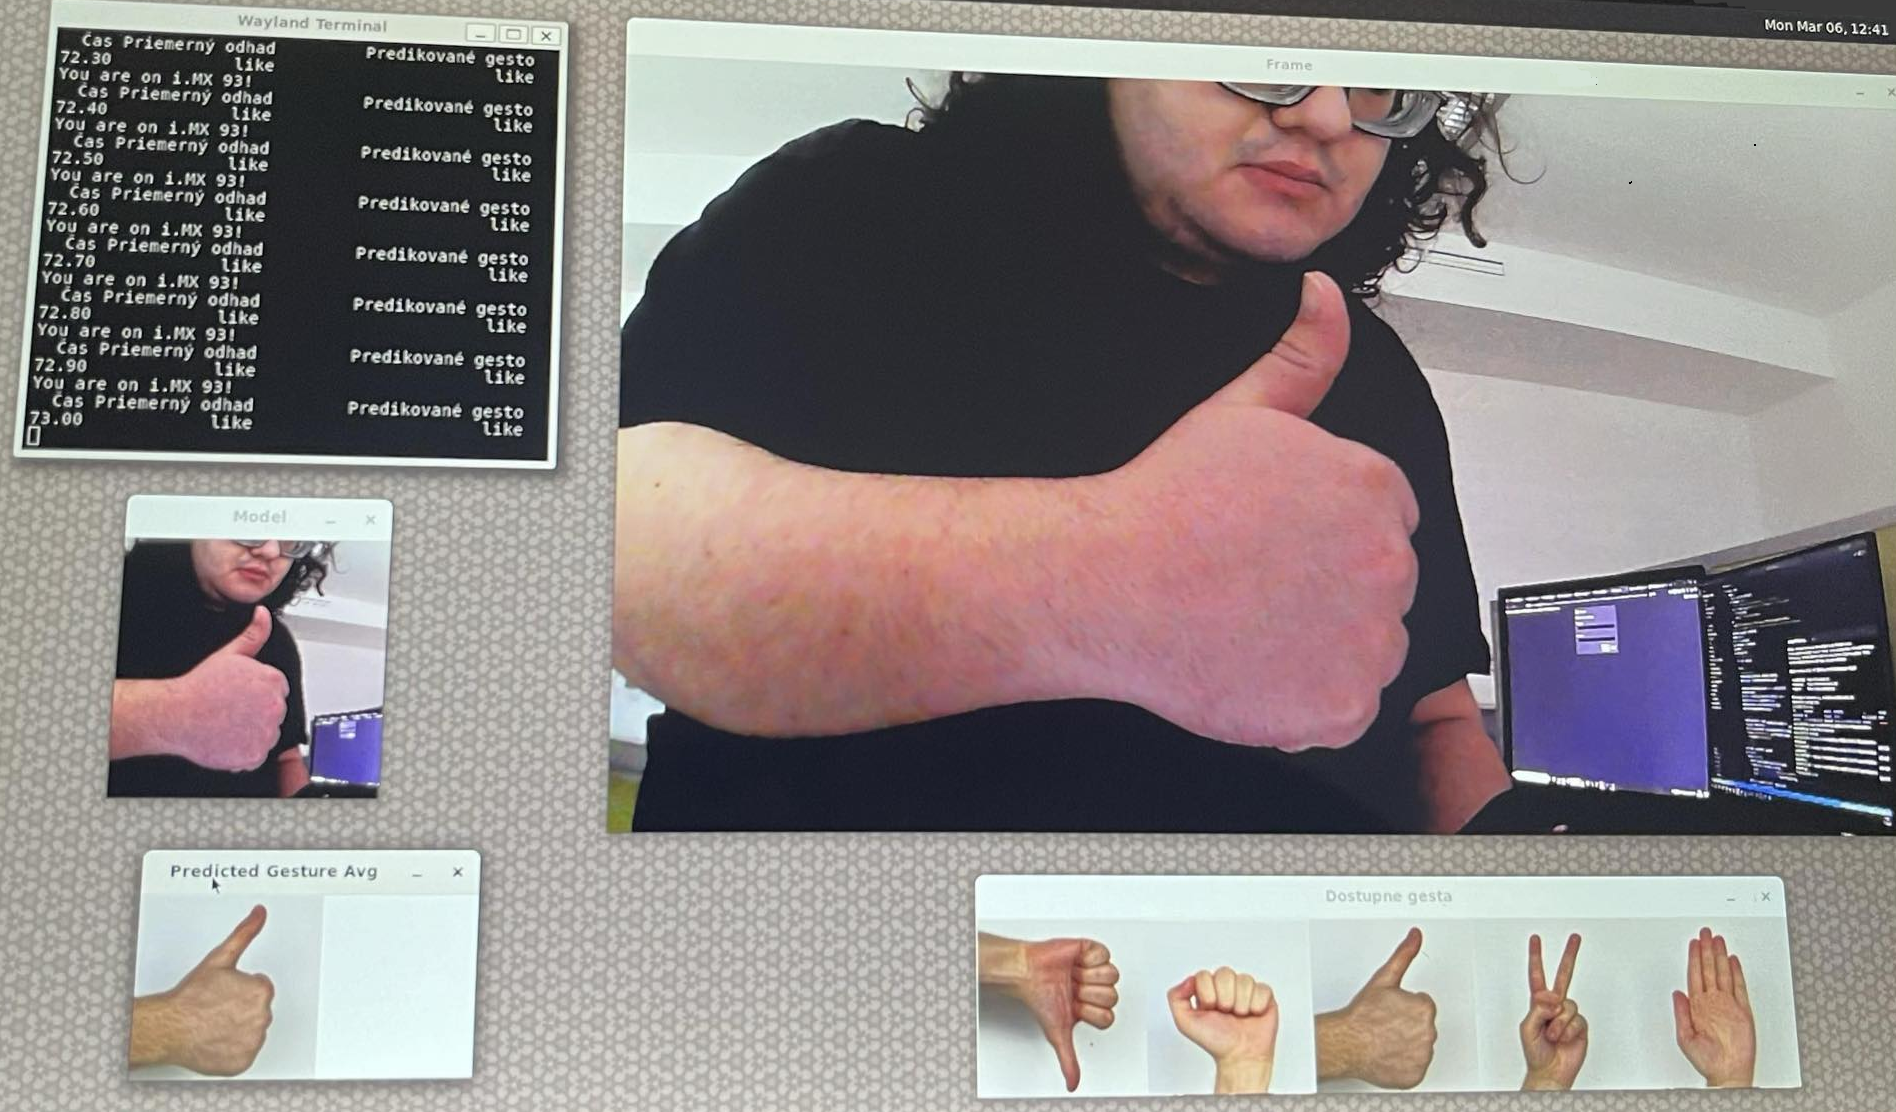
\includegraphics[width=\textwidth]{obrazky-figures/me_gesturing.png}
\caption{Graphical user interface of the demonstration application.}
\label{fig:ui_demo}
\end{figure}

\chapter{Testing}
\section{Performance of Training Process}
Training was performed on a 5600x AMD CPU with 32GB of RAM. The dataset consisted of 100 images per gesture for training across five different gestures, with a validation set of 20 images per gesture. The batch size was set to 32.

For MobileNetV2, training one epoch took approximately 30 seconds. This efficiency can be attributed to the fact that only the top layers of the model were being trained, while the rest of the pre-trained layers were frozen. This approach reduces the number of trainable parameters, significantly speeding up the training process without compromising the model’s ability to generalize well from the learned ImageNet features.

In contrast, training one epoch for EfficientDet Lite 2 took about 15 minutes. This longer duration is due to the model's architecture and the need to train more layers from scratch compared to MobileNetV2.

\section{Performance of Inference Process}
During inference, various performance metrics were continuously recorded to monitor and optimize the efficiency of the system \ref{code:inference_measuring_example}. The primary metrics included cycle times, preprocess times, inference times, memory usage, and model accuracy.

\subsection{Real-Time Performance Data Collection}
To gather precise data on the performance of the application, specific global variables were initialized to store times and usage statistics:

\begin{itemize}
    \item \textbf{Cycle Times}: Time taken for each complete loop of processing, including capturing, preprocessing, inference, and logging.
    \item \textbf{Preprocess Times}: Time required to preprocess each frame before feeding it to the model.
    \item \textbf{Inference Times}: Duration of the model inference per frame.
    \item \textbf{Memory Usages}: Memory consumption measured after each inference cycle.
    \item \textbf{Model Accuracies}: Accuracy of the model's predictions collected after each inference execution.
\end{itemize}

\newpage
After completing each cycle, these times and statistics were measured using the Python `time` library for time measurements and `subprocess` for memory usage as shown in the following script segment.


\begin{figure}[H]
\begin{lstlisting}[language=Python]
import time
import subprocess

# Example of logging a cycle time
start_cycle_time = time.time()
# Operations...
cycle_time = time.time() - start_cycle_time
cycle_times.append(cycle_time)

# Memory usage example
memory_usage = get_memory_usage()
memory_usages.append(memory_usage)

def get_memory_usage():
    try:
        mem_usage = subprocess.check_output(['free', '-m']).decode('utf-8').split('\n')
        used_memory = mem_usage[1].split()[2]
        return int(used_memory)
    except:
        return -1

# Model certainty example
# Confidence of detected objects
probabilities = interpreter.get_tensor(output_details[0]['index'])[0]
probabilities = probabilities * 100
probability = probabilities[0]
model_accuracies.append(probability)
\end{lstlisting}
\caption{Data collection}
\label{code:inference_measuring_example}
\end{figure}

\subsection{Logging Data}
After the script was finished inferring, either by reaching the end of an input video file or, if inference is running from a video camera, by pressing the key ''q'', the performance data was logged in the log file, providing a historical record for later analysis \ref{code:inference_logging_example}.

\begin{figure}[H]
\begin{lstlisting}[language=Python]
import datetime
def log_performance_metrics():
    current_time = datetime.datetime.now().strftime("%Y-%m-%d_%H-%M-%S")
    log_filename = f"logs/{GRAPH_NAME}_{current_time}.log"

    average_cycle_time = sum(cycle_times) / len(cycle_times)
    average_preprocess_time = sum(preprocess_times) / len(preprocess_times)
    average_inference_time = sum(inference_times) / len(inference_times)
    average_memory_usage = sum(memory_usages) / len(memory_usages)
    average_accuracy = sum(model_accuracies) / len(model_accuracies)

    with open(log_filename, 'w') as log_file:
        log_entry = f"Time: {current_time}\n" +
                    f"Avg. Cycle Time: {average_cycle_time:.8f}s\n" +
                    f"Avg. Preprocess Time: {average_preprocess_time:.8f}s\n" +
                    f"Avg. Inference Time: {average_inference_time:.8f}s\n" +
                    f"Avg. Memory Usage: {average_memory_usage} MB\n" +
                    f"Avg. Accuracy: {average_accuracy:.2f}%\n"
        log_file.write(log_entry)
\end{lstlisting}
\caption{Data logging}
\label{code:inference_logging_example}
\end{figure}

This comprehensive logging strategy ensures that all relevant performance data are captured, enabling ongoing monitoring and optimization of the application's performance.

\subsection{Analyzing Data}
To ensure consistency in the evaluation of model performance, a single video, available in the `src` folder on the GitHub repository \cite{gajdosik2024gesture} with the name `video\_test.mp4`, was used for testing all models. This approach guarantees that all models are tested under identical conditions, enabling a fair comparison of their inference performance.

\subsubsection{Testing Setup}
The models tested include the non-quantized MobileNetV2, the natively quantized EfficientDet Lite 2, and the EfficientDet Lite 2 optimized for NPU using Vela Tool. The video capture setup was standardized using a script that ensures that the gesture is correctly displayed for all models by preprocessing the frames to the required dimensions. The relevant preprocessing steps were referenced in a previous section (see \ref{code:mobilenetv2_preprocess}). The hardware used in the tests includes the NXP i.MX 93 board \cite{iMX93FAMFS} and the personal computer with 32 GB of ram and 5600x AMD CPU.

\subsubsection{Inference Performance Results}
The performance data collected during the tests are summarized as follows \ref{tab:performance_metrics}:

\begin{table}[h]
\centering
\caption{Performance Metrics of Different Models on Various Platforms on average}
\resizebox{\textwidth}{!}{%
\begin{tabular}{lccccccc}
\toprule
\textbf{Model} & {Quantization} & {Platform} & {Epochs} & \textbf{Cycle Time (ms) $\downarrow$} & \textbf{Preprocess Time (ms) $\downarrow$} & \textbf{Inference Time (s) $\downarrow$} & \textbf{Memory Usage (MB) $\downarrow$} & \textbf{Accuracy (\%) $\uparrow$} \\
\midrule
MobileNetV2 & No & x64 & 20 & 15 & 0.4 & 11 & 2228 & 73.01 \\
EfficientDet Lite 2 & No & x64 & 60 & 131 & 1.6 & 128 & 2051 & 74.08 \\
EfficientDet Lite 2 & Yes & x64 & 20 & 133 & 0.51 & 131 & 729 & 69.71 \\
EfficientDet Lite 2 & Yes & x64 & 5 & 135 & 0.57 & 133 & 636 & 30.41 \\
MobileNetV2 & No & i.MX93 & 20 & 220 & 13 & 157 & 367 & 76.61 \\
EfficientDet Lite 2 & Yes & i.MX93 & 20 & 754 & 18 & 679 & 364 & 71.73 \\
EfficientDet Lite 2 & NPU & i.MX93 & 20 & 239 & 15 & 169 & 369 & 64.28 \\
\bottomrule
\end{tabular}%
}
\label{tab:performance_metrics}
\end{table}



\subsubsection{Analysis and Conclusion}
The porting of EfficientDet Lite 2 to an NPU via Vela Tool significantly improved the cycle time, showing a marked decrease compared to the non-optimized quantized model. Although there is a slight decrease in accuracy, the benefits of reduced cycle time and lower latency are evident, highlighting the advantage of using NPU optimization for real-time applications. This improvement demonstrates the potential for NPUs to improve performance in scenarios where rapid processing is crucial.

Moreover, despite not being quantized or NPU-optimized, MobileNetV2 exhibited the best cycle time and the highest accuracy among the tested models. This outcome suggests that MobileNetV2 is inherently well designed for efficient processing and accuracy. All models were trained with the same amount of data, which underscores the inherent efficiency of MobileNetV2's architecture.

Additionally, it is important to note that the MobileNetV2 model was also run on a high-performance desktop PC, used as a baseline to understand the upper limits of processing efficiency under optimal conditions. Inference on an i.MX or other ARM-based platform is expected to be slower due to the less powerful hardware, although the accuracy of the model's predictions should not significantly differ.

These results illustrate the effectiveness of hardware-specific optimizations and the impact of quantization and NPU deployment on the performance metrics of deep learning models. They also highlight the inherent strengths of MobileNetV2's design, which seems to excel even without specialized hardware optimizations.


\section{Methodology and Preparation for User Testing}
User testing of the demonstration application was carried out in two main settings to evaluate its usability and effectiveness. The demonstration application employed MobilNetV2 as this model had the best ratio of accuracy with inference time. The first setting involved internal tests among colleagues at the NXP branch in Brno, who are well-educated individuals from technical faculties such as Faculty of Information Technology, Faculty of Electrical Engineering and Communication and Faculty of Mechanical Engineering from Brno University of Technology. The second phase of testing occurred during a presentation at ''perFEKT JobFair 2024'' \ref{fig:nxp_booth_demo} with NXP on April 24, 2024, where the application was demonstrated to students primarily from the Faculty of Electrical Engineering and Communication of Brno University of Technology, as well as various visitors and competitors from the IT industry.

\subsection{Internal Developer Testing}
The purpose of this phase was to provide insight and constructive feedback on user interface design and overall user experience from the developer's point of view. Colleagues were asked to interact with the application and suggest enhancements that could make it more intuitive and effective for end users. Feedback from this phase was instrumental in identifying features that could enhance user satisfaction, such as the inclusion of confidence scores to provide transparency about the model's certainty in its predictions. This internal review was crucial to refining the user interface and usability of the application before it was introduced to a wider audience.

\subsection{Public User Testing at perFEKT JOBFAIR 2024}
The second phase took place during the ''perFEKT JobFair 2024''\footnote{This image has been included with the consent of the individuals depicted.} \ref{fig:nxp_booth_demo} with NXP on April 24, 2024. Here, the application was presented to a diverse group of attendees. This public demonstration served as a platform to assess the usability and effectiveness of the application from an end-user point of view. Feedback was primarily focused on user experience, interface design, and overall user satisfaction. This event provided valuable information on how potential users interact with the application in a real-world scenario.

\begin{figure}[H]
\centering
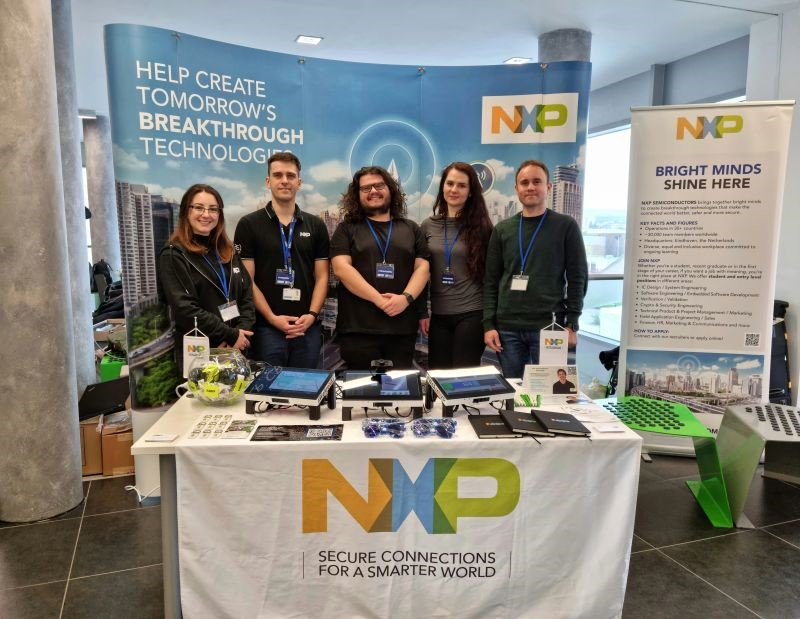
\includegraphics[width=\textwidth]{obrazky-figures/JOBFAIR FEKT.jpg}
\caption{The demonstration application presented at the NXP booth during perFEKT JOBFAIR 2024. Visible in the center of the table is the application being demonstrated, with myself and colleagues.}
\label{fig:nxp_booth_demo}
\end{figure}

\section{Evaluation of User Reactions and Feedback}
Feedback from users highlighted several areas for improvement. Key points included the need for enhancing the model's accuracy, as the model struggled in a new untested scenario with various light sources which in combination of displaying currently predicted gesture resulted in rapid switching between various gestures as the model struggled to be confident in only one gesture and oscilated between 2 to 3 different ones. Also, users were initially confused by the dual-camera displays, not realizing that the smaller window was where the model expects gestures to be directed for accurate recognition. In addition, there was strong interest in how confident the model was in its predictions.

\subsection{Enhancements to Graphical Display}
In the latest version of the demonstration application \cite{gajdosik2024gesture}, significant enhancements have been made to improve the user interface and functionality. One major improvement is the consolidation of the camera display windows. The application has been redesigned to show only one window, the one that the model uses to view and analyze gestures. This window has been enlarged to provide a clearer view of the gestures being demonstrated, making it easier for users to interact accurately with the inference application. In addition, confidence scores have been included in the predicted gesture display and along with each gesture in the gesture recognition overview. This feature significantly aids both users and developers by providing a quantitative measure of the model's certainty in its predictions. The enhancement of the display setup helps mitigate previous user confusion and improves the overall usability of the application.

\chapter{Conclusion}
\section{Project Challenges}

One of the main challenges faced in the project was the initial inefficiency in the training process. Improving the training required iterative adjustments, fine-tuning the model, and optimizing the script for better performance. The quality of training was highly dependent on the learning rate, the loss function used, and, particularly, on factors such as batch size and dataset size.

Another significant challenge was the unsuccessful attempt to quantify the MobileNetV2 model. Despite various efforts, the quantization of MobileNetV2 was not successful, which prevented the testing and evaluation of the model's performance and accuracy after quantization. This issue necessitated the use of an alternative model, the EfficientDet Lite 2, which was successfully quantized and used for further experiments. The inability to quantize MobileNetV2 highlighted the need to select appropriate models for specific hardware optimizations and the potential limitations of certain architectures when it comes to deploying them on resources-constrained devices.

\section{Future Work}

The development and testing of the gesture recognition system have shown promising results in terms of performance and accuracy. However, several opportunities for enhancement remain that could further improve the system's effectiveness and broaden its practical applications.

\begin{itemize}
    \item \textbf{Utilization of Docker Containers:} To address the challenges associated with package installations and dependencies, particularly for the EfficientDet Lite 2 model, future iterations could leverage Docker containers. This approach would standardize the development environment, reducing setup times and eliminating inconsistencies across different platforms.
    
    \item \textbf{Enhanced Data Augmentation:} Increasing the diversity and volume of training data through more sophisticated data augmentation techniques could significantly improve model robustness and accuracy. Preprocessing the input to simplify the data for the model could also enhance its ability to generalize from the training data to real-world scenarios.

    \item \textbf{Advanced Image Preprocessing:} Currently, the input from the camera is used as captured without additional preprocessing modifications. To further enhance the model's performance and robustness, implementing advanced image preprocessing techniques could be beneficial. Techniques such as converting images to grayscale, adjusting contrast, or applying filters to emphasize specific features could significantly simplify the visual data. This simplification can help the model focus on essential gestures by reducing background noise and variations in lighting conditions.
    
    \item \textbf{Application Control Integration:} While the current application primarily serves as a demonstration tool, integrating control functionalities to manipulate real-world objects or software systems could vastly increase its utility. This would transform the system from a proof-of-concept into a practical tool for interactive technology.
    
    \item \textbf{Exploring Alternative Model Architectures:} Future research should also explore and compare various deep learning architectures. Experimenting with different hyperparameters, training strategies, and datasets could provide insights into optimal configurations for speed and accuracy. This comparative analysis would help identify the most effective models for gesture recognition.
\end{itemize}

  \else
    \input{projekt-01-kapitoly-chapters}
  \fi
  
  % Kompilace po částech (viz výše, nutno odkomentovat a zakomentovat input výše)
  % Compilation piecewise (see above, it is necessary to uncomment it and comment out input above)
  %\subfile{chapters/projekt-01-uvod-introduction}
  % ...
  %\subfile{chapters/projekt-05-zaver-conclusion}

  % Pouzita literatura / Bibliography
  % ----------------------------------------------
\ifslovak
  \makeatletter
  \def\@openbib@code{\addcontentsline{toc}{chapter}{Literatúra}}
  \makeatother
  \bibliographystyle{bib-styles/Pysny/skplain}
\else
  \ifczech
    \makeatletter
    \def\@openbib@code{\addcontentsline{toc}{chapter}{Literatura}}
    \makeatother
    \bibliographystyle{bib-styles/Pysny/czplain}
  \else 
    \makeatletter
    \def\@openbib@code{\addcontentsline{toc}{chapter}{Bibliography}}
    \makeatother
    \bibliographystyle{bib-styles/Pysny/enplain}
  %  \bibliographystyle{alpha}
  \fi
\fi
  \begin{flushleft}
  \bibliography{projekt-20-literatura-bibliography}
  \end{flushleft}

  % vynechani stranky v oboustrannem rezimu
  % Skip the page in the two-sided mode
  \iftwoside
    \cleardoublepage
  \fi

  % Prilohy / Appendices
  % ---------------------------------------------
  \appendix
\ifczech
  \renewcommand{\appendixpagename}{Přílohy}
  \renewcommand{\appendixtocname}{Přílohy}
  \renewcommand{\appendixname}{Příloha}
\fi
\ifslovak
  \renewcommand{\appendixpagename}{Prílohy}
  \renewcommand{\appendixtocname}{Prílohy}
  \renewcommand{\appendixname}{Príloha}
\fi
%  \appendixpage

% vynechani stranky v oboustrannem rezimu
% Skip the page in the two-sided mode
%\iftwoside
%  \cleardoublepage
%\fi
  
\ifslovak
%  \section*{Zoznam príloh}
%  \addcontentsline{toc}{section}{Zoznam príloh}
\else
  \ifczech
%    \section*{Seznam příloh}
%    \addcontentsline{toc}{section}{Seznam příloh}
  \else
%    \section*{List of Appendices}
%    \addcontentsline{toc}{section}{List of Appendices}
  \fi
\fi
  \startcontents[chapters]
  \setlength{\parskip}{0pt} 
  % seznam příloh / list of appendices
  % \printcontents[chapters]{l}{0}{\setcounter{tocdepth}{2}}
  
  \ifODSAZ
    \setlength{\parskip}{0.5\bigskipamount}
  \else
    \setlength{\parskip}{0pt}
  \fi
  
  % vynechani stranky v oboustrannem rezimu
  \iftwoside
    \cleardoublepage
  \fi
  
  % Přílohy / Appendices
  \ifenglish
    \input{projekt-30-prilohy-appendices-en}
  \else
    \input{projekt-30-prilohy-appendices}
  \fi
  
  % Kompilace po částech (viz výše, nutno odkomentovat)
  % Compilation piecewise (see above, it is necessary to uncomment it)
  %\subfile{projekt-30-prilohy-appendices}
  
\end{document}
